\section{Results}

\begin{table}[t]
\centering\small
\caption{\textbf{Size-matched subcircuits and the analyses each supports.}
Networks are induced subgraphs grown by breadth-first expansion and stripped of
degree-zero nodes. The final column records whether synaptic valence is available:
in the MICrONS release used here every annotated inhibitory soma is disconnected,
and diffusion tractography carries no valence at all, so neither network can support
sign-attributed motif analysis.}
\label{tab:datasets}
\resizebox{\columnwidth}{!}{%
\begin{tabular}{llrrrrrc}
\toprule
\textbf{Network} & \textbf{Species} & \textbf{$N$} & \textbf{$|E|$} &
\textbf{Dens.\ (\%)} & \textbf{$\bar{k}$} & \textbf{Inh.\ (\%)} & \textbf{Valence} \\
\midrule
\textit{C. elegans} & C. elegans & 300 & 5,044 & 5.62 & 16.8 & 8.7 & yes \\
\textit{Drosophila} CX & D. melanogaster & 400 & 7,856 & 4.92 & 19.6 & 45.5 & yes \\
\textit{Drosophila} AL & D. melanogaster & 400 & 16,468 & 10.32 & 41.2 & 29.8 & yes \\
Mouse V1 L2/3 & M. musculus & 334 & 1,734 & 1.56 & 5.2 & 0.0 & \textbf{no} \\
Human HCP & H. sapiens & 400 & 6,092 & 3.82 & 15.2 & 0.0 & \textbf{no} \\
\bottomrule
\end{tabular}}
\end{table}

\begin{table*}[t]
\centering\small
\caption{\textbf{Every experiment in this study.} Counts are read from each experiment's
own output file at build time rather than transcribed, so the table cannot disagree with
what was run; an experiment whose output is absent is reported as absent. This list is the
same one the accompanying documentation prints, generated from a single source. The unit
differs by row --- a ``run'' is one network at one rung trained to convergence, an
``evaluation'' one network at one operating point probed for one metric --- so the totals
are not comparable across rows and are not summed.}
\label{tab:experiments}
\begin{tabular}{@{}l p{0.70\textwidth} r@{}}
\toprule
\textbf{Section} & \textbf{Experiment} & \textbf{Size} \\
\midrule
\S\ref{sec:res-motifs} & Are the classic subgraphs really over-represented? Exact sign-attributed counts against 500 degree-preserving surrogates per network. & 35 tests \\
\S\ref{sec:res-null} & Validation of the annealed chain: does it hit the target census, does it actually randomise, and does it leave untargeted structure alone? & 5 networks \\
\S\ref{sec:res-robust} & The same ensemble redrawn over a factor-of-eight range of chain lengths and from both possible starting points, ruling out two ways a sampler could fake the result. & 200 draws \\
\S\ref{sec:res-protocol} & What does the benchmark measure? Includes the reservoir with its recurrent matri$\times$ set to zero, under both readout protocols. & 8 conditions \\
\S\ref{sec:res-ladder} & L0 density to L4 real connectome on spoken digits, each rung adding exactly one structural property; accuracy, memory capacity, kernel and generalisation rank. & 375 runs \\
\S\ref{sec:res-rate} & The same decomposition with every network recalibrated to a common firing rate, because matching spectral radius does not match activity. & 250 runs \\
\S\ref{sec:res-ladder} & Does taking a size-matched subgraph of a larger connectome bias the degree result? Run because the ladder depends on the extraction being neutral. & 5 networks \\
\S\ref{sec:res-nullchoice} & The headline experiment. Both readings of ''degree-preserving randomisation'' against both unit models across nine gains, on the original toolbox's own connectomes. & 2,700 evaluations \\
\S\ref{sec:res-nullchoice} & Structural descriptors of both ensembles against the real graph, including the prediction that they must coincide on an unweighted network. & 105 graphs \\
\S\ref{sec:res-unit} & Input gain $\times$ threshold $\times$ leak, searching for the configuration that would refute our own spiking result rather than the one that confirms it. & 1,728 evaluations \\
\S\ref{sec:res-operating} & The whole decomposition across the critical region, because a comparison at one gain is a statement about that gain. & 1,400 evaluations \\
\S\ref{sec:res-operating} & Locating the published advantage on the gain axis at matched spectral radius. & 2,500 evaluations \\
\S\ref{sec:res-dynamics} & The same decomposition measured on task-independent probes, so the ordering does not depend on one benchmark. & 250 runs \\
\S\ref{sec:res-degeneracy} & Random, hub-targeted and adversarial edge removal, testing whether the operational alignment predicts how much damage a direction does. & 540 prunings \\
\S\ref{sec:res-hardware} & Real logic synthesis and technology mapping of the accompanying RTL, reporting only what the open flow can establish. & 4 designs \\
\bottomrule
\end{tabular}
\end{table*}


Table~\ref{tab:experiments} lists every experiment reported below with its size, counted
from its own output file. We give it up front because the argument of this paper is
cumulative --- no single comparison in it is decisive, and several of them contradict each
other by design.

\subsection{Motif enrichment, recomputed}
\label{sec:res-motifs}

We first re-establish the empirical starting point on the size-matched subcircuits of
Table~\ref{tab:datasets}, using $K = \NMotifNulls$ degree-preserving surrogates
per network (resolution floor $p \ge \MotifPFloor$) and exact counts throughout.

\begin{figure*}[t]
\centering
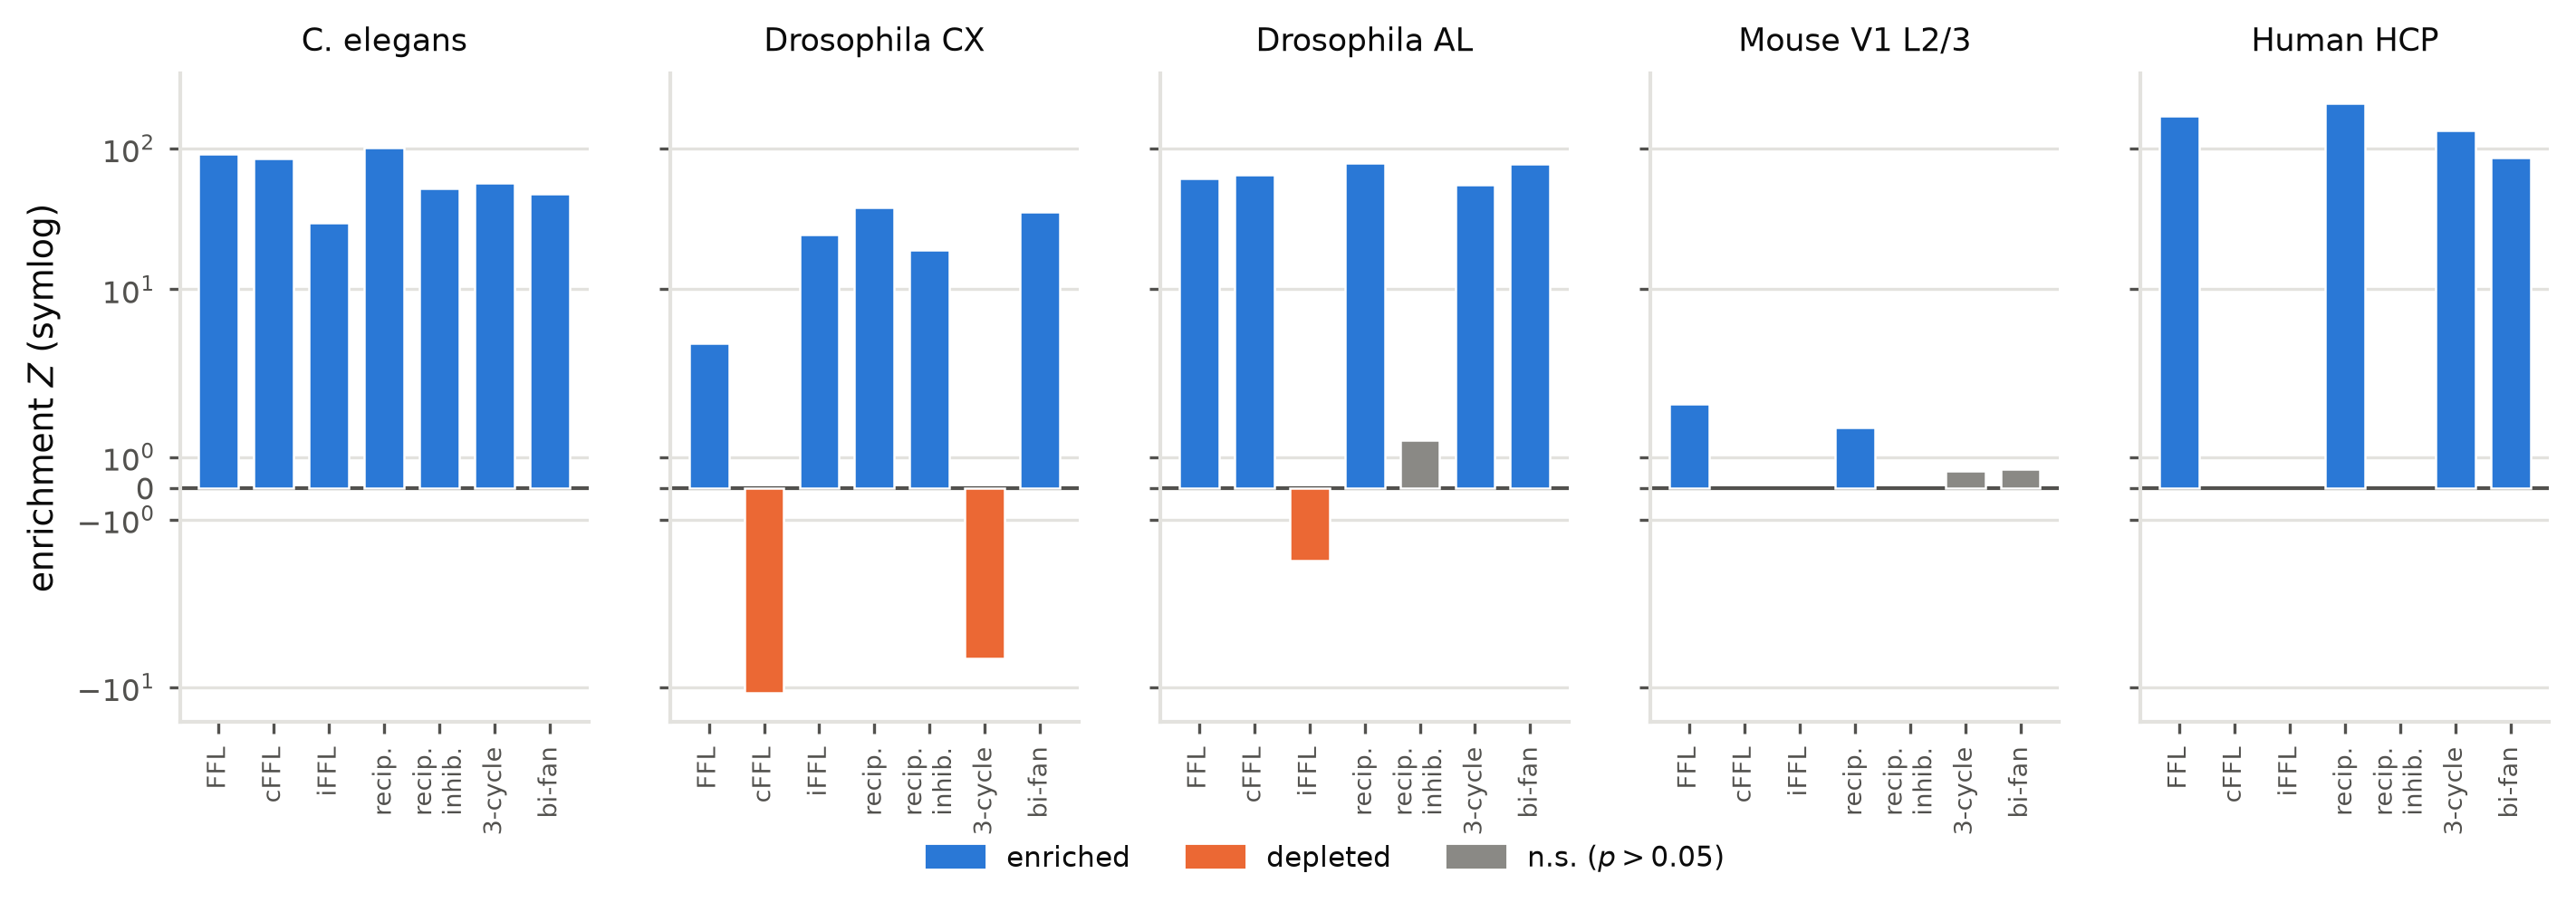
\includegraphics[width=0.95\textwidth]{figures/fig_motifs.png}
\caption{\textbf{Motif enrichment against a degree-preserving null}, $K = \NMotifNulls$
surrogates per network, exact counts, symlog axis. Colour encodes the outcome of each
test rather than the network, because the point is that the outcome differs between
networks: the \textit{Drosophila} central complex \emph{depletes} coherent feedforward
loops and directed 3-cycles, the antennal lobe depletes incoherent feedforward loops,
and mouse V1 L2/3 is close to its null throughout. Bars appear only where the dataset
supports the motif's definition --- coherent and incoherent feedforward loops require
synaptic valence, which diffusion tractography does not carry and which the mouse
release does not supply in connected form. The human column's magnitudes reflect an
almost entirely reciprocal tractography graph rather than a stronger biological effect
(see text).}
\label{fig:motifs}
\end{figure*}

Enrichment is real and often large, but it is not uniform, and the recomputation does
not support the description of these motifs as conserved across phylogeny. Of the
$\NMotifTests$ interpretable (network, motif) tests, $\NMotifEnriched$ are significantly
enriched, $\NMotifDepleted$ are significantly \emph{depleted}, and $\NMotifNull$ are
indistinguishable from the degree-preserving null.

Figure~\ref{fig:motifs} shows the pattern. In \textit{C. elegans} every motif is
strongly enriched: feedforward loops reach
$Z = \ZCeleFfl$ and reciprocal pairs $Z = \ZCeleRecip$. The \textit{Drosophila} central
complex breaks the pattern in the coordinate the motif literature cares about most ---
its coherent feedforward loops are depleted, $Z = \ZDrosCXCffl$, against an enrichment
of $\ZCeleCffl$ in the worm --- while its reciprocal pairs remain enriched
($Z = \ZDrosCXRecip$) and its directed 3-cycles are depleted ($Z = \ZDrosCXCyc$). Mouse
V1 L2/3 is the clearest case: no motif in that network is enriched by more than
$Z = \ZMouseFfl$, and directed 3-cycles ($Z = \ZMouseCyc$) and bi-fans are
indistinguishable from chance. Correspondingly, the normalised significance profiles of
the two sign-attributed fly circuits agree with each other no better than either agrees
with the worm ($\SPFlyFly$ for fly--fly, against $\SPWormFly$ and $\SPWormFlyAL$ for
worm--fly), so what is conserved is not a profile shape but the presence of some excess
somewhere.

Four qualifications belong with these numbers rather than in a footnote. First,
sign-attributed motifs are reported only for \textit{C. elegans} and \textit{Drosophila};
for the mouse and human networks the coherent and total feedforward loop counts would be
equal by construction (\S\ref{sec:data}), so quoting a coherent-FFL enrichment there
reports a topological result under a biological name. Second, the enrichment is measured
against a degree-preserving ensemble, and because Dale's principle is automatically
preserved by double-edge swaps, no part of this enrichment can be attributed to
excitatory/inhibitory organisation. Third, the very large $Z$-scores in the human row
($Z = \ZHumanFfl$ for feedforward loops) should not be read as a stronger biological
result than the invertebrate ones: HCP tractography is an essentially undirected
network, in which almost every edge is reciprocal, and a degree-preserving null of such
a graph is a poor match for it in ways that have nothing to do with computation. Fourth,
and most importantly for what follows: overrepresentation is a statement about a graph,
not about a computation. The remainder of the paper asks what, if anything, it buys.

\subsection{The motif-preserving ensemble}
\label{sec:res-null}

\begin{table*}[t]
\centering\small
\caption{\textbf{Validation of the motif-preserving ensemble.} The chain must hit its
target census, genuinely randomise, and not reproduce structure it was not asked to
preserve. Columns 2--3: worst-case relative error across the six targeted motif counts,
and the fraction of chains meeting the 2\% convergence criterion. Columns 4--5: edge
overlap with the empirical connectome for the motif-matched (L3) and degree-matched
(L2) ensembles --- L3 is close to the unconstrained level, so it is not the
connectome in disguise. Columns 6--7: mean pairwise overlap \emph{between} ensemble
members, as evidence of mixing. L3 members are somewhat less mutually distinct than L2
members, which is expected because the constrained set is a subset of the unconstrained
one; what matters is that they remain far from identical, so the chain explores the
constraint surface rather than collapsing onto one region of it. This is empirical
evidence of adequate mixing, not a proof of uniform sampling. Columns 8--10: bi-fan
counts, a 4-node motif deliberately excluded from the objective, reproduced neither in
value nor in a consistent direction, confirming the chain constrains 3-node structure
specifically rather than reconstructing the graph.}
\label{tab:nullval}
\resizebox{\textwidth}{!}{%
\begin{tabular}{lrrrrrrrrr}
\toprule
& \multicolumn{2}{c}{\textbf{Target match}} & \multicolumn{2}{c}{\textbf{Overlap w/ real (\%)}}
& \multicolumn{2}{c}{\textbf{Pairwise overlap (\%)}}
& \multicolumn{3}{c}{\textbf{Held-out bi-fan count}} \\
\cmidrule(lr){2-3}\cmidrule(lr){4-5}\cmidrule(lr){6-7}\cmidrule(lr){8-10}
\textbf{Network} & \textbf{max err (\%)} & \textbf{conv.\ (\%)} & \textbf{L3} & \textbf{L2}
& \textbf{L3} & \textbf{L2} & \textbf{empirical} & \textbf{L3} & \textbf{L2} \\
\midrule
\textit{C. elegans} & 0.3 & 100 & 13.9 & 11.6 & 21.0 & 11.1 & 118,612 & 179,732 & 65,882 \\
\textit{Drosophila} CX & 0.2 & 100 & 20.5 & 19.9 & 22.4 & 20.4 & 824,107 & 647,161 & 573,668 \\
\textit{Drosophila} AL & 0.1 & 100 & 43.9 & 40.0 & 45.6 & 38.9 & 12,622,936 & 12,038,186 & 9,058,482 \\
Mouse V1 L2/3 & 0.9 & 100 & 10.6 & 10.7 & 10.7 & 10.4 & 5,826 & 5,930 & 5,594 \\
Human HCP & 0.5 & 100 & 11.4 & 7.8 & 20.3 & 7.9 & 129,726 & 243,934 & 46,585 \\
\bottomrule
\end{tabular}}
\end{table*}


Table~\ref{tab:nullval} reports the three properties the annealed ensemble has to have
simultaneously. The chains reach the empirical census to within
$\AnnealErrCeleVal$ worst-case relative error on \textit{C. elegans} across all six
targeted motif counts, and converge on every network in the set, while retaining only
$\OverlapCele$ edge overlap with the empirical connectome --- against
$\OverlapLtwoCele$ for an unconstrained degree-preserving rewiring. The motif-matched surrogates are therefore not the
connectome in disguise: they agree with it on the motif census and are otherwise as
randomised as a standard null.

The held-out statistic confirms that the constraint is specific. Bi-fan counts, a
4-node motif deliberately excluded from the annealing objective, are not reproduced by
the L3 ensemble, and --- the point that matters --- they are not even displaced in a
consistent direction. In \textit{C. elegans} the empirical count is $\BifanRealCele$
against $\BifanLthreeCele$ for the motif-matched ensemble, an overshoot; in the
\textit{Drosophila} central complex it is $\BifanRealDrosCX$ against
$\BifanLthreeDrosCX$, an undershoot. Constraining the 3-node census therefore neither
fixes nor systematically biases 4-node structure. The chain constrains exactly the
structure whose contribution the ladder is designed to isolate and leaves higher-order
structure free, which is what distinguishes L3 from a partial reconstruction of the
connectome.

One further property is worth stating because the whole rung depends on it: the
constraint has to be \emph{binding}. If the empirical census were within ordinary
sampling range of the unconstrained ensemble, L3 would be a relabelled L2 and the
L2\,$\rightarrow$\,L3 contrast would be measuring nothing. It is not: the enrichment
$Z$-scores of \S\ref{sec:res-motifs} are the distance between exactly these two
ensembles' censuses, and they run from $Z = \ZMouseFfl$ in the least-enriched network to
$Z = \ZHumanRecip$ in the most. Except in mouse V1, where the census is close to its null
by construction and the contrast is correspondingly uninformative, L2 and L3 are
separated by tens to hundreds of null standard deviations in the coordinates the chain
constrains.

One asymmetry should be stated rather than left to the table. The L3 ensemble's members
are somewhat more similar to \emph{each other} than the unconstrained ensemble's members
are (mean pairwise edge overlap $\PairwiseLthreeCele$ against
$\PairwiseLtwoCele$ in \textit{C. elegans}), which is expected --- a constrained set is
smaller than the set that contains it --- but it means the L3 rung has less ensemble
diversity than L2 at equal instance count. We report the pairwise overlap for every
network so that this is visible, and we note that it works against detecting an L2--L3
difference only by inflating L3's variance, not by suppressing a mean difference.

\subsection{Protocol sensitivity}
\label{sec:res-protocol}

Before comparing rungs we fix what the benchmark can detect. Under an all-to-all
protocol, a reservoir with its recurrent matrix set to zero scores $\ZeroRecFull$ on
SHD while the \textit{C. elegans} connectome scores $\ZeroRecFullConn$: the recurrent
matrix is not used, and no structural comparison run in that regime can be informative.
Under the sensory/motor-disjoint protocol used throughout this paper, the same
zero-recurrence control falls to $\ZeroRecSplit$ against a chance level of
$\ChanceLevel$, while the connectome reaches $\ZeroRecSplitConn$. Task-relevant signal
must now traverse the recurrent graph, so differences between networks are attributable
to wiring.

\subsection{Decomposing performance across the ladder}
\label{sec:res-ladder}

\begin{table*}[t]
\centering\small
\caption{\textbf{SHD test accuracy (\%) by ladder rung}, mean $\pm$ 95\% CI over
15 surrogates per rung. Every rung is matched on node count, edge count, spectral
radius and input projection; adjacent rungs differ in exactly one structural
property. Chance is 5.0\%; a zero-recurrence network scores \ZeroRecSplit{} under
this protocol.}
\label{tab:ladder_acc}
\resizebox{\textwidth}{!}{%
\begin{tabular}{lrrrrr}
\toprule
\textbf{Rung} & \textit{C. elegans} & \textit{Drosophila} CX & \textit{Drosophila} AL & Mouse V1 L2/3 & Human HCP \\
\midrule
L0 density & 37.1\,$\pm$\,1.0 & 42.7\,$\pm$\,0.6 & 39.9\,$\pm$\,1.3 & 39.8\,$\pm$\,1.0 & 38.8\,$\pm$\,0.7 \\
L1 $+$degree & 36.8\,$\pm$\,1.1 & 38.0\,$\pm$\,1.3 & 31.9\,$\pm$\,1.9 & 32.1\,$\pm$\,1.9 & 39.1\,$\pm$\,1.2 \\
L2 $+$valence & 36.9\,$\pm$\,1.1 & 34.8\,$\pm$\,1.5 & 30.6\,$\pm$\,1.7 & 31.5\,$\pm$\,1.9 & 38.3\,$\pm$\,1.5 \\
L3 $+$motifs & 33.1\,$\pm$\,1.4 & 33.9\,$\pm$\,1.6 & 27.1\,$\pm$\,2.7 & 31.8\,$\pm$\,1.4 & 32.4\,$\pm$\,1.4 \\
L4 connectome & 36.3\,$\pm$\,1.7 & 26.3\,$\pm$\,2.0 & 28.2\,$\pm$\,1.6 & 31.8\,$\pm$\,1.8 & 38.6\,$\pm$\,1.0 \\
\bottomrule
\end{tabular}}
\end{table*}

\begin{table}[t]
\centering\small
\caption{\textbf{Contribution of each structural property}, as the difference between
adjacent ladder rungs in SHD accuracy (percentage points), with percentile-bootstrap
95\% CIs, Hedges' $g$, and Holm-corrected $p$-values across the whole family of
contrasts. $\ast$ marks $p_{\mathrm{Holm}} < 0.05$.}
\label{tab:contrasts}
\resizebox{\columnwidth}{!}{%
\begin{tabular}{llrlrr}
\toprule
\textbf{Network} & \textbf{Property added} & \textbf{$\Delta$ (pp)} &
\textbf{95\% CI} & \textbf{$g$} & \textbf{$p_{\mathrm{Holm}}$} \\
\midrule
\textit{C. elegans} & + degree sequence & -0.29 & [-1.78, +1.11] & -0.14 & 1.000 \\
\textit{C. elegans} & + valence placement & +0.15 & [-1.40, +1.70] & +0.07 & 1.000 \\
\textit{C. elegans} & + motif census & -3.80 & [-5.54, -2.04] & -1.46 & 0.005$\ast$ \\
\textit{C. elegans} & Empirical connectome & +3.16 & [+1.01, +5.24] & +0.99 & 0.115 \\
\textit{Drosophila} CX & + degree sequence & -4.65 & [-6.12, -3.36] & -2.31 & 0.000$\ast$ \\
\textit{Drosophila} CX & + valence placement & -3.16 & [-5.02, -1.29] & -1.14 & 0.045$\ast$ \\
\textit{Drosophila} CX & + motif census & -0.98 & [-3.13, +1.11] & -0.31 & 1.000 \\
\textit{Drosophila} CX & Empirical connectome & -7.60 & [-10.05, -5.07] & -2.04 & 0.000$\ast$ \\
\textit{Drosophila} AL & + degree sequence & -8.02 & [-10.35, -5.85] & -2.38 & 0.000$\ast$ \\
\textit{Drosophila} AL & + valence placement & -1.28 & [-3.72, +1.30] & -0.34 & 1.000 \\
\textit{Drosophila} AL & + motif census & -3.50 & [-6.70, -0.50] & -0.76 & 0.465 \\
\textit{Drosophila} AL & Empirical connectome & +1.06 & [-1.85, +4.23] & +0.24 & 1.000 \\
Mouse V1 L2/3 & + degree sequence & -7.65 & [-9.66, -5.65] & -2.51 & 0.000$\ast$ \\
Mouse V1 L2/3 & + valence placement & -0.63 & [-3.21, +1.96] & -0.16 & 1.000 \\
Mouse V1 L2/3 & + motif census & +0.30 & [-1.99, +2.59] & +0.09 & 1.000 \\
Mouse V1 L2/3 & Empirical connectome & +0.02 & [-2.21, +2.24] & +0.01 & 1.000 \\
Human HCP & + degree sequence & +0.34 & [-0.97, +1.69] & +0.18 & 1.000 \\
Human HCP & + valence placement & -0.82 & [-2.59, +1.02] & -0.31 & 1.000 \\
Human HCP & + motif census & -5.94 & [-7.96, -4.00] & -2.06 & 0.000$\ast$ \\
Human HCP & Empirical connectome & +6.25 & [+4.61, +7.90] & +2.52 & 0.000$\ast$ \\
\bottomrule
\end{tabular}}
\end{table}


\begin{figure*}[t]
\centering
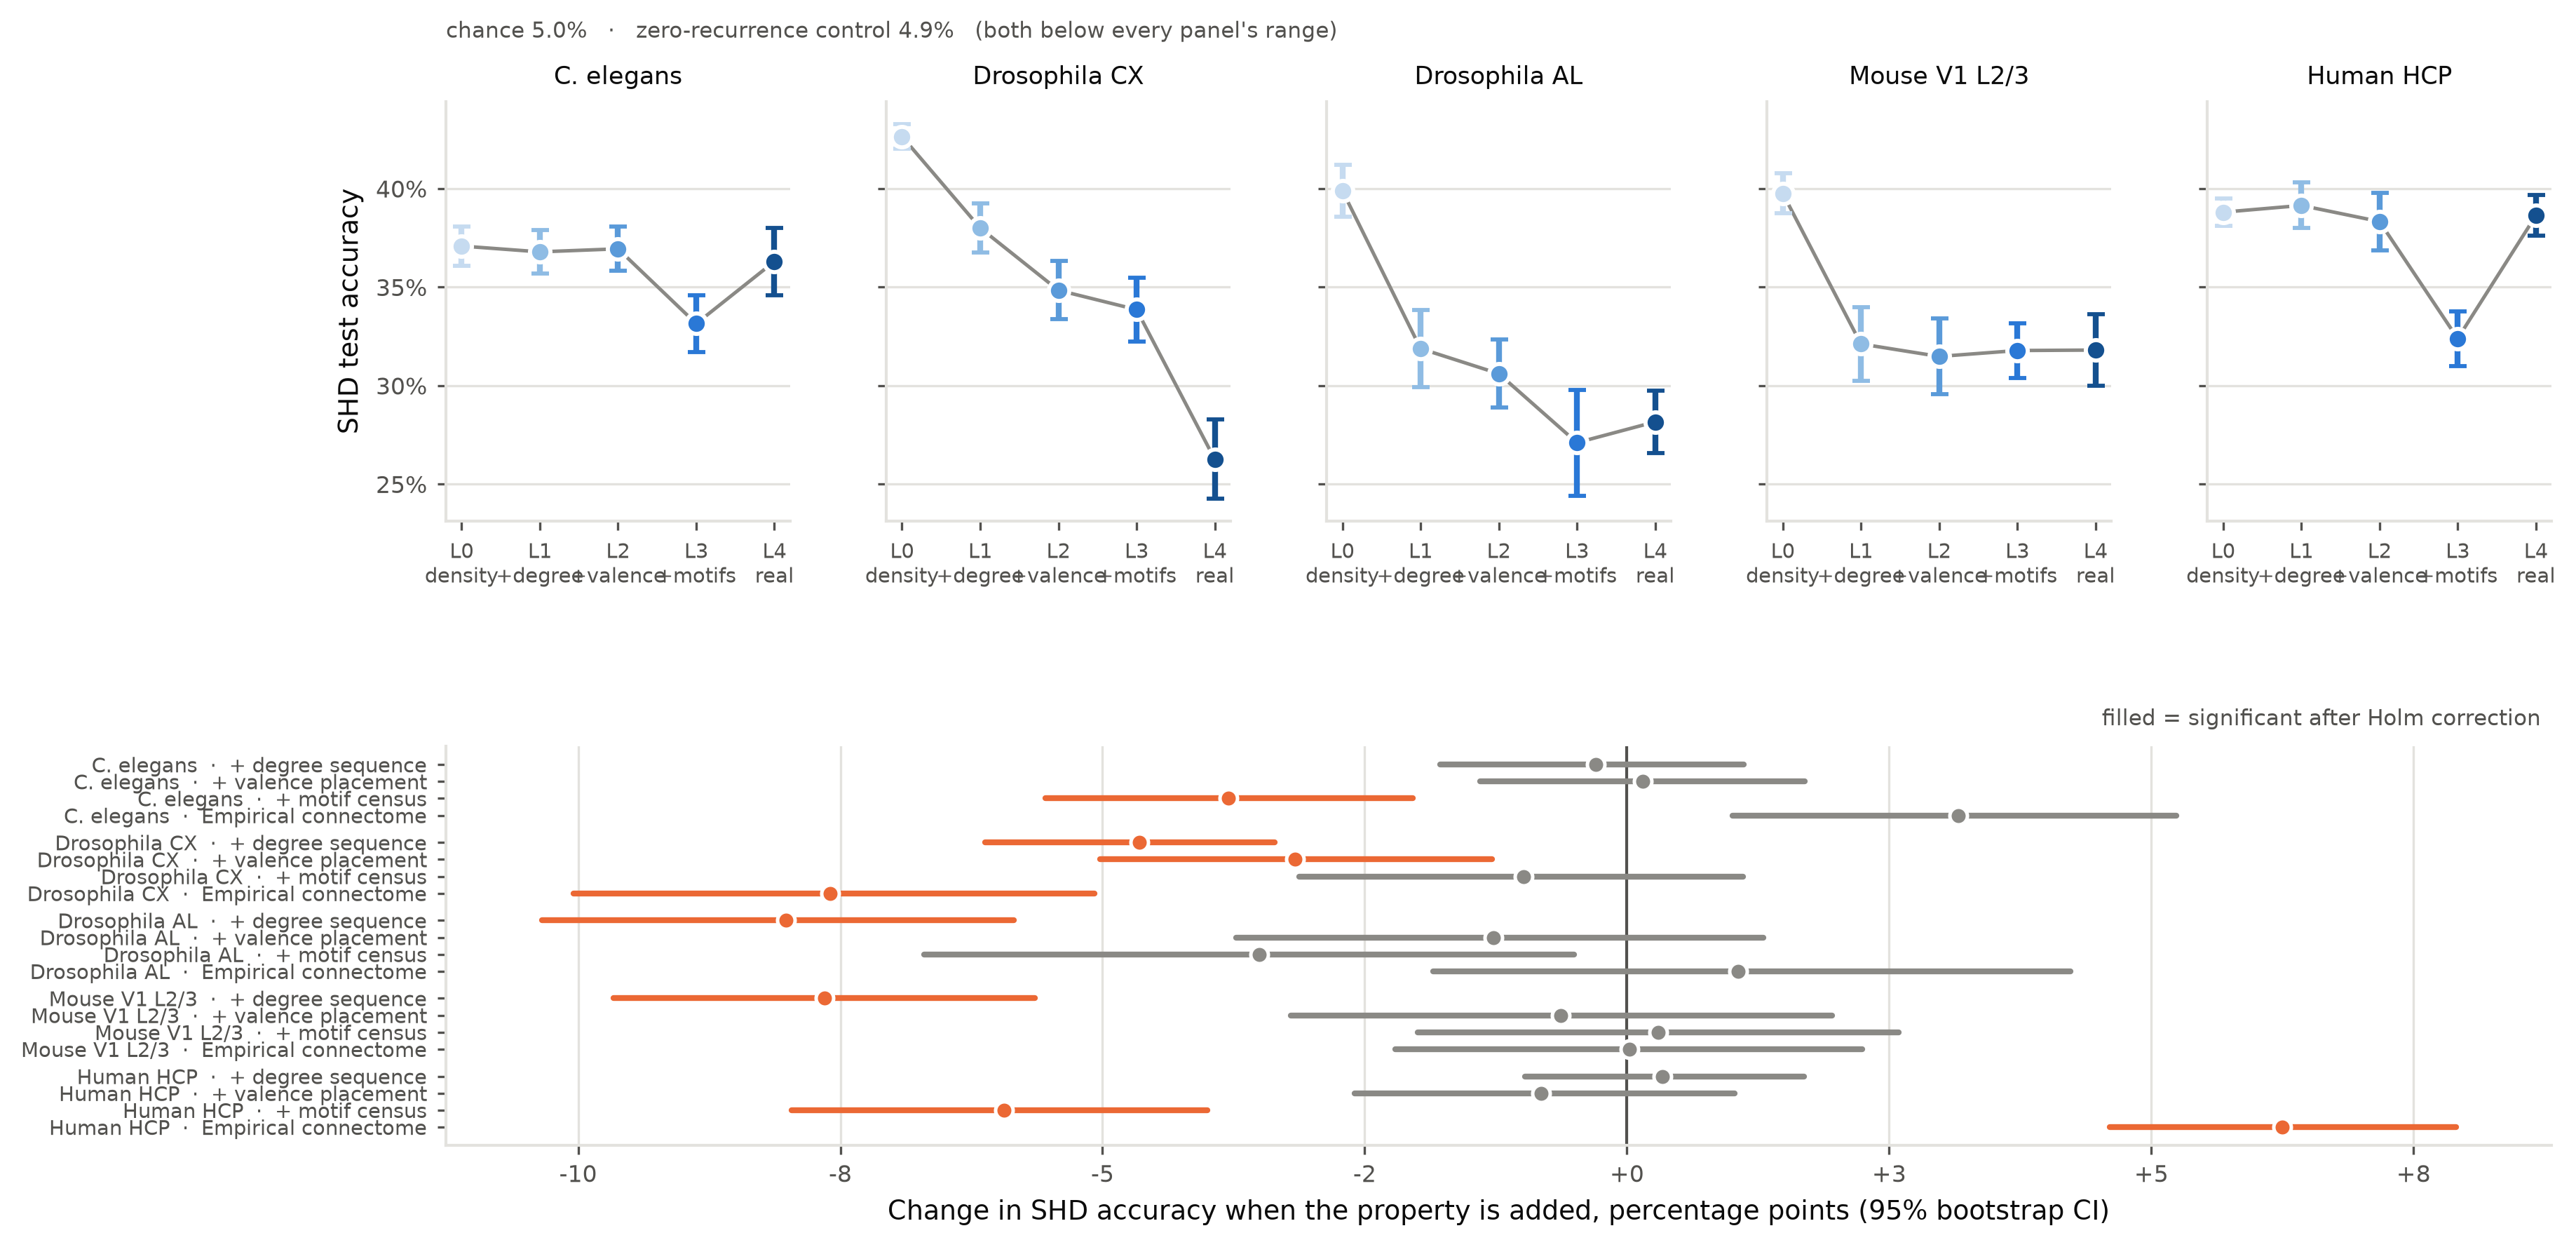
\includegraphics[width=0.95\textwidth]{figures/fig_ladder.png}
\caption{\textbf{Structural decomposition of reservoir performance on SHD.}
\textbf{Top:} mean accuracy with 95\% CIs at each ladder rung, per network. Each rung
adds one structural property to the rung on its left; all rungs are matched on node
count, edge count, spectral radius and input projection. Dotted line, chance; dashed
line, the zero-recurrence control. \textbf{Bottom:} the contribution of each property,
as the difference between adjacent rungs with bootstrap 95\% CIs; intervals spanning
zero indicate a property that does not measurably change performance.}
\label{fig:ladder}
\end{figure*}

Table~\ref{tab:ladder_acc} and Figure~\ref{fig:ladder} give the decomposition. We read it
property by property rather than as a count over the $\NLadderContrasts$ contrasts,
because the question is not how many differences reach significance but which structural
properties this benchmark is sensitive to and in which direction.

The direction is the first thing to say, because it is uniform and it is not the
direction the motif hypothesis predicts. \emph{Every} structural property that
measurably moves accuracy moves it \emph{down}. Each rung adds something the connectome
has and the rung below it does not, and at every step where the effect is resolvable the
addition makes the network a worse reservoir.

\textbf{Degree sequence} (L0\,$\rightarrow$\,L1) is the largest single contributor:
significant after Holm correction in $\NDegreeSig$ of $\NDegreeTotal$ networks, median
effect $\DegreeEffectMedian$, largest $\DegreeEffectMax$ (Hedges'
$g = \DegreeEffectMaxG$).

\textbf{The motif census} (L2\,$\rightarrow$\,L3) is the contrast this paper was built to
measure: it adds the connectome's exact 3-node motif spectrum while holding degree
sequence and valence placement fixed, using the ensemble validated in
\S\ref{sec:res-null}. It is significant in $\NMotifSig$ of $\NMotifTotal$ networks, with
median effect $\MotifEffectMedian$ and largest $\MotifEffectMax$
($g = \MotifEffectMaxG$). This is not a negligible effect and we do not report it as
one --- it is comparable in size to the degree-sequence contrast --- but its sign is
negative. Imposing a connectome's motif structure on a degree- and valence-matched
surrogate costs accuracy on this task.

\textbf{Valence placement} (L1\,$\rightarrow$\,L2) --- returning inhibitory labels to the
neurons that carry them rather than permuting them across the graph --- is significant in
$\NValenceSig$ of $\NValenceTotal$, median $\ValenceEffectMedian$.

\textbf{The residual wiring} (L3\,$\rightarrow$\,L4) adds everything else about the
empirical graph: weights aside, its exact synapse-by-synapse identity. Significant in
$\NResidualSig$ of $\NResidualTotal$, median $\ResidualEffectMedian$, and it is the one
property whose sign is not consistent --- it helps in some networks and hurts in others.

\paragraph{What the design could have detected.}
A small measured effect and an underpowered design look identical in a table, so we state
the bound. With $\NinstancesLadder$ surrogates per rung and $\NLadderContrasts$ contrasts
in the family, the design has $\PowerLevel$ power to resolve a standardised effect of
$d = \MDEUncorrected$ uncorrected and $d = \MDEHolm$ at the Holm worst case. The
significant contrasts reported above sit at or beyond that bound; the non-significant
ones do not exclude moderate effects, and we do not claim they do.

\paragraph{The reading.}
The motif hypothesis, as we stated it in \S\ref{sec:intro} and as our own earlier work
asserted it, is that connectome motif structure confers a computational advantage over
matched controls. On this benchmark, in the fixed-reservoir regime, at matched size,
density, spectral radius and input projection, it does not. The measured effect of adding
the empirical motif census has the opposite sign, and it is large enough to detect in two
of five networks.

We are careful about what this licenses, because the uniform negative sign across
properties is itself informative about the probe. A reservoir with a linear decoder
rewards distributed, high-dimensional state. Connectome structure --- heavy-tailed degrees,
excess feedforward loops and reciprocal pairs --- concentrates and correlates activity,
which spends the dimensions such a decoder needs. That is a property of this probe as
much as of these graphs, and a different task with a different readout could order them
differently. What it does establish is that an Erd\H{o}s--R\'enyi comparison cannot be
used to argue the motif hypothesis on this benchmark, because that comparison comes out
against it.

\subsection{The ladder at a matched operating point}
\label{sec:res-rate}

\begin{table*}[t]
\centering\small
\caption{\textbf{The ladder at a matched operating point.} Each network is calibrated
individually, by bisection on its own spectral radius, to a common mean firing rate of
0.07; 10 surrogates per rung.
\textbf{Top:} SHD test accuracy (\%), mean $\pm$ 95\% CI, over the surrogates that
reached the target. \textbf{Bottom:} the spectral radius each topology required, averaged
over all surrogates including those that did not. 27 of
250 surrogates never reached the target rate: the bisection
saturates at the top of its bracket and the network still fires below target.
$^{\ast}$ marks a cell where some surrogates were excluded on that ground and
$\dagger$ one where all were --- the \textit{Drosophila} central complex is 66\%
inhibitory, so raising its gain raises its inhibition and its attainable rate is capped.
Accuracy differences that survive in Table~\ref{tab:ladder_acc} but not here were
differences in activity level rather than in wiring.}
\label{tab:rate_matched}
\resizebox{\textwidth}{!}{%
\begin{tabular}{lrrrrr}
\toprule
\textbf{Rung} & \textit{C. elegans} & \textit{Drosophila} CX & \textit{Drosophila} AL & Mouse V1 L2/3 & Human HCP \\
\midrule
\multicolumn{6}{l}{\emph{Test accuracy (\%)}} \\
L0 density & 39.0\,$\pm$\,1.2 & 41.9\,$\pm$\,0.6 & 42.0\,$\pm$\,0.8 & 41.0\,$\pm$\,0.9 & 41.0\,$\pm$\,1.2 \\
L1 $+$degree & 37.1\,$\pm$\,1.6 & 37.9\,$\pm$\,1.3 & 32.7\,$\pm$\,2.8 & 32.8\,$\pm$\,1.9 & 38.2\,$\pm$\,0.8 \\
L2 $+$valence & 36.1\,$\pm$\,1.3 & 35.1\,$\pm$\,1.9$^{\ast}$ & 31.0\,$\pm$\,1.7 & 32.4\,$\pm$\,1.9 & 38.6\,$\pm$\,1.1 \\
L3 $+$motifs & 35.0\,$\pm$\,1.4$^{\ast}$ & 39.0\,$\pm$\,5.0$^{\ast}$ & 28.6\,$\pm$\,2.2 & 32.8\,$\pm$\,1.8 & 34.3\,$\pm$\,1.4$^{\ast}$ \\
L4 connectome & 35.9\,$\pm$\,1.9 & $\dagger$ & 28.1\,$\pm$\,1.9 & 32.0\,$\pm$\,2.3 & 38.9\,$\pm$\,0.8 \\
\midrule
\multicolumn{6}{l}{\emph{Calibrated spectral radius $\rho$}} \\
L0 density & 1.22 & 1.15 & 1.12 & 1.15 & 1.17 \\
L1 $+$degree & 1.28 & 1.62 & 1.26 & 1.25 & 1.28 \\
L2 $+$valence & 1.26 & 5.96 & 1.36 & 1.23 & 1.28 \\
L3 $+$motifs & 1.41 & 5.79 & 1.38 & 1.21 & 1.46 \\
L4 connectome & 1.30 & 6.00 & 1.35 & 1.25 & 1.31 \\
\bottomrule
\end{tabular}}
\end{table*}


\begin{figure*}[t]
\centering
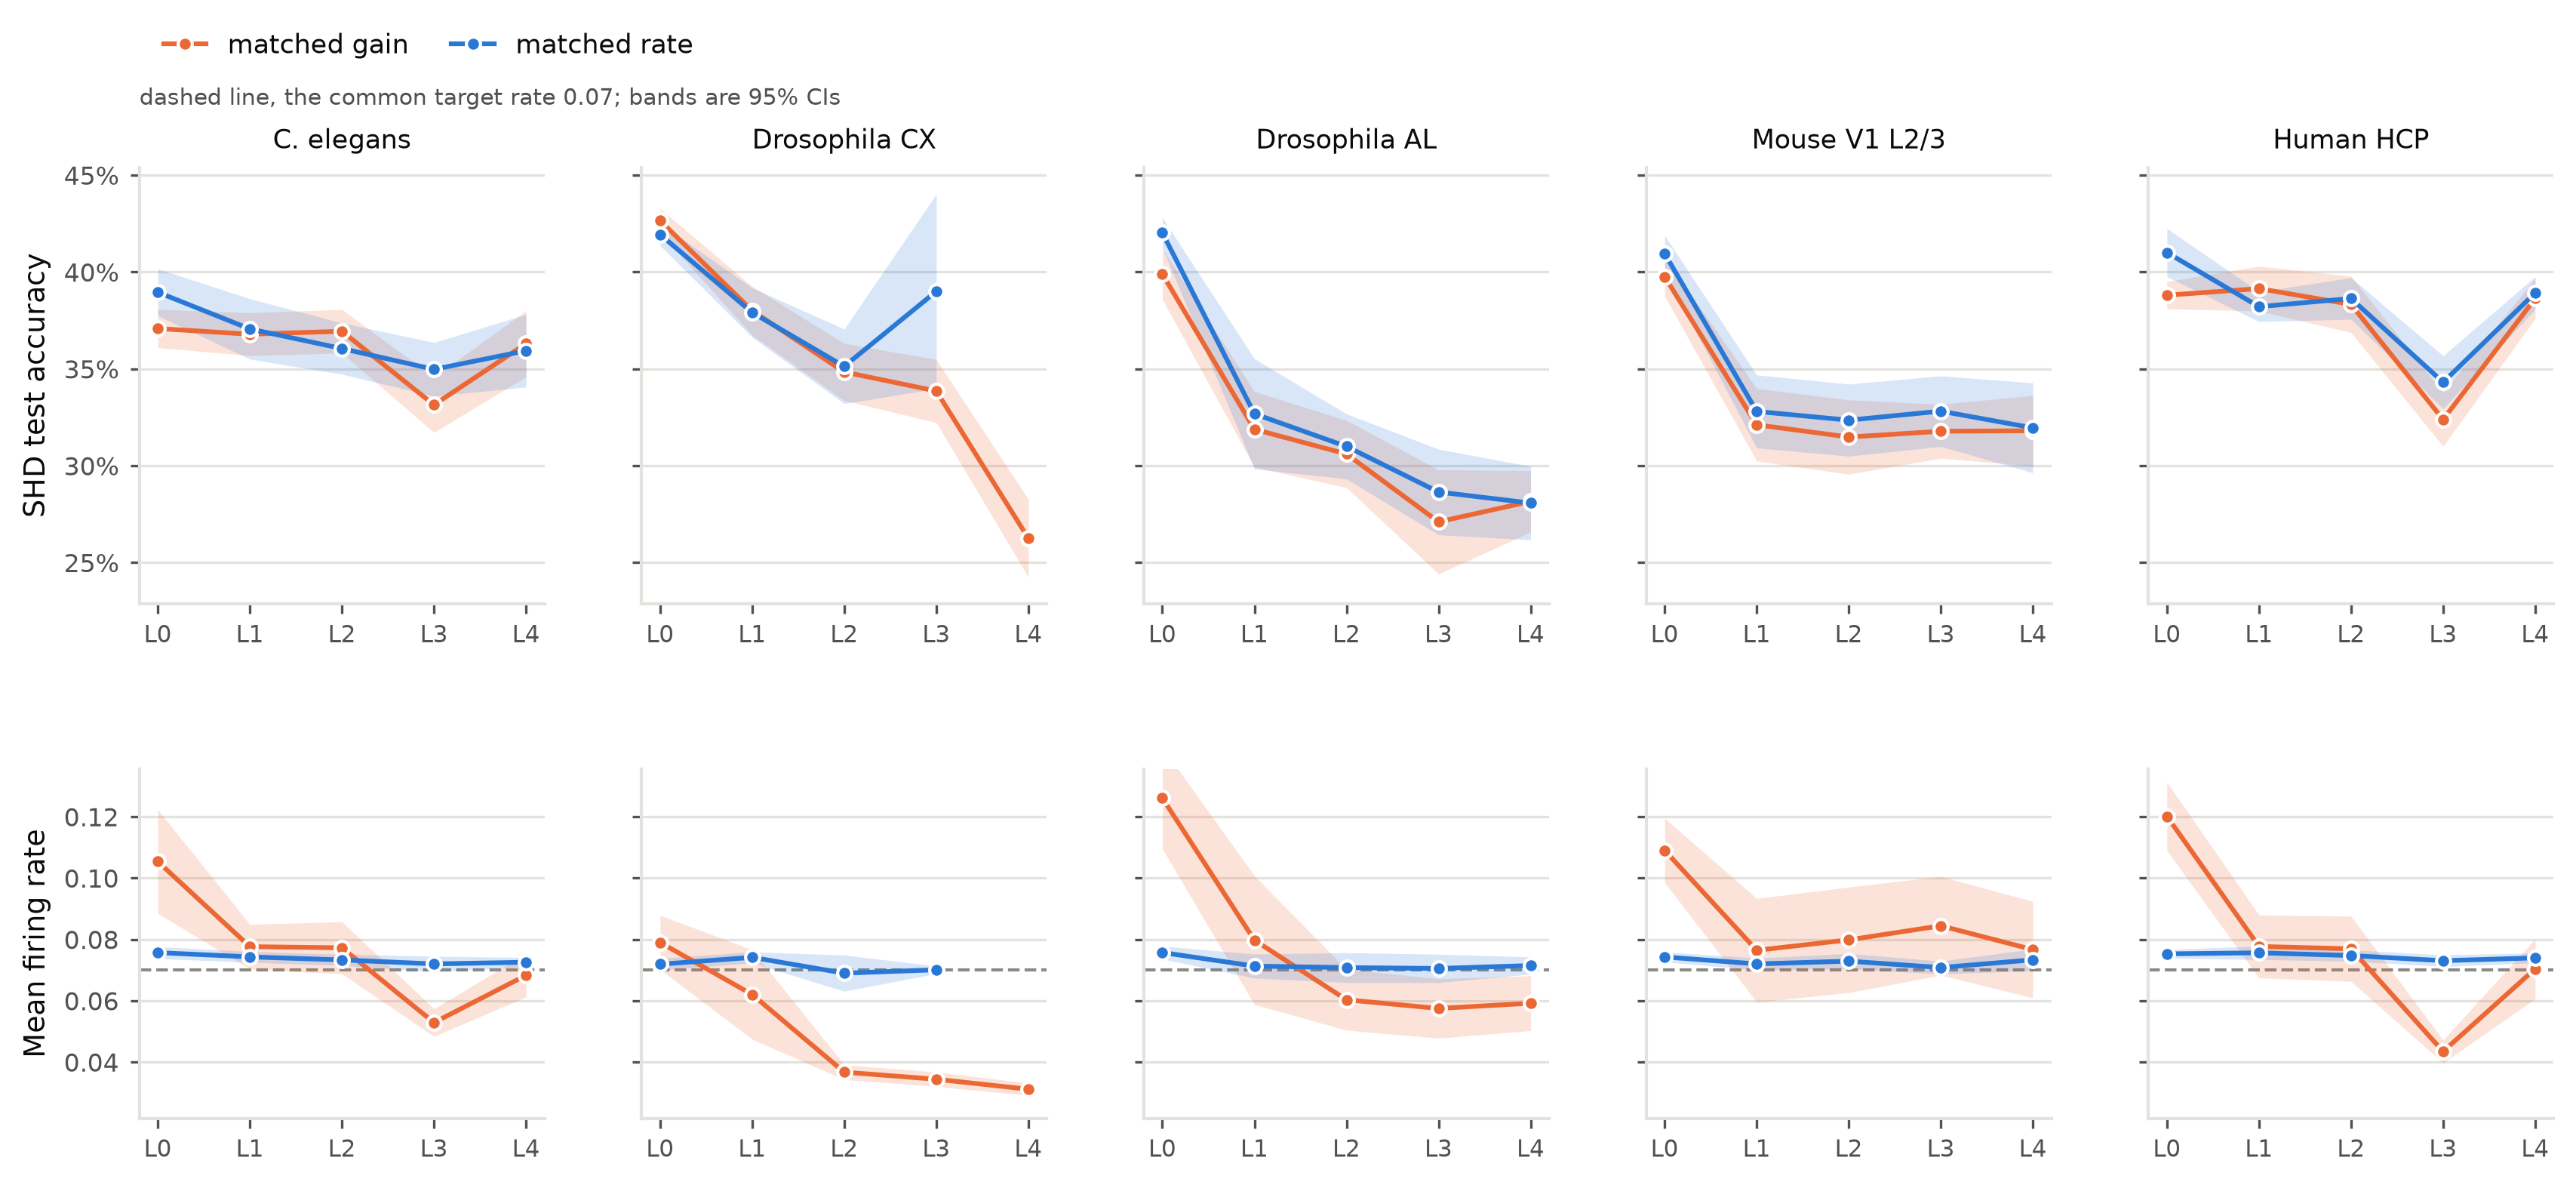
\includegraphics[width=0.95\textwidth]{figures/fig_rate_matched.png}
\caption{\textbf{The ladder at matched gain and at a matched operating point.} Colour
encodes the matching regime rather than the network, because the comparison is within a
network. Rungs are L0 density, L1 $+$degree, L2 $+$valence, L3 $+$motifs, L4 the
empirical connectome. \textbf{Top:} SHD test accuracy by rung under each regime.
\textbf{Bottom:}
mean firing rate. At a fixed spectral radius (orange) the rungs run at different rates,
and the accuracy ordering tracks the rate; calibrating each network individually to the
common rate (blue, dashed line) holds every network on the target. The accuracy decline
from L0 to L4 survives that correction. Cells whose calibration never reached the target
are omitted from the matched-rate series, which is why the \textit{Drosophila} CX panel
has no L4 point. Bands are 95\% CIs.}
\label{fig:rate_matched}
\end{figure*}

One asymmetry in Table~\ref{tab:ladder_acc} needs separating out before any of it can
be read as a statement about topology. The rungs are matched on spectral radius, but
they do not fire at the same rate: averaged over networks the Erd\H{o}s--R\'enyi rung
settles at $\RateLzero$ mean rate against $\RateLfour$ for the empirical connectome, a
factor of $\RateRatioLzeroLfour$. Across all runs firing rate is correlated with accuracy
($r = \RateAccCorr$), and it determines the synaptic-operation count outright. A
comparison at matched gain therefore confounds topology with operating point, in the
direction that flatters the unstructured control.

Recalibrating each network individually to a common mean rate of $\TargetRate$ removes
the confound, at the cost of letting spectral radius vary. Table~\ref{tab:rate_matched}
and Figure~\ref{fig:rate_matched} give the result, and it is not the one we expected.

\paragraph{Where the calibration fails, and why that is a result.}
Of $\NRateCells$ calibrated surrogates, $\NRateUnmatched$ never reach the target rate at
all: the bisection saturates at the top of its bracket and the network still fires below
target, in the worst case at $\RateUnmatchedWorst$ of it. $\NRateUnmatchedThere$ of the
$\NRateUnmatched$ are in one network, $\RateUnmatchedWhere$, whose edges are 66\%
inhibitory --- raising the gain in such a circuit raises its inhibition too, so its
attainable firing rate is bounded above by its own valence organisation. The effect
strengthens down the rungs, from none at L0 and L1 to every surrogate at L4, which
places the ceiling squarely on the empirical valence placement rather than on density. We exclude those cells from every matched-rate
statistic rather than averaging them in, since a cell that was not calibrated is not
rate-matched, and we report the exclusion because the ceiling is a property of the
network worth stating. That leaves $\NRateCompleteNetworks$ networks in which every rung
is fully matched, and the contrasts below are computed on those.

\paragraph{The operating point does not explain the gap.}
At a matched operating point the Erd\H{o}s--R\'enyi rung still outperforms the empirical
connectome, by $\RmLzeroMinusLfourMin$ to $\RmLzeroMinusLfour$ of accuracy in
percentage points, against
$\MgLzeroMinusLfourMin$ to $\MgLzeroMinusLfour$ for the same networks at matched gain.
The gap does not shrink; it is marginally larger. Firing rate is therefore a real
confound in the matched-gain comparison --- it is why we report both --- but it is not
what produces the unstructured control's advantage, and we were wrong to expect that it
would.

What the two versions together establish is narrower and firmer than either alone. On
this task, in this regime, connectome wiring is not merely no better than an
unstructured graph of the same size and density: it is measurably worse, and that
remains true when the networks are compared at the same activity level. Reading down the
rungs shows where the cost is incurred. The step that imposes the empirical degree
sequence, L0\,$\rightarrow$\,L1, accounts for $\RmDegreeShareMin$ to
$\RmDegreeShareMax$ of the whole decline; the three steps that follow --- adding valence
placement, the motif census and the remaining wiring --- divide the rest between them and
are individually small. Degree heterogeneity, not motif structure, is the
structural property this benchmark is sensitive to --- and its effect has the opposite
sign to the one the motif literature would predict for connectome structure as a whole.

We are explicit about what this does not show. It does not show that connectome wiring
is bad for computation, but that a degree-heterogeneous graph is a poor fixed reservoir
for a 20-class classification with a linear readout, which is one task in one regime and
not the objective any nervous system is under selection for. It does show that a
comparison against an Erd\H{o}s--R\'enyi control cannot be used to argue that connectome
structure confers a computational advantage, because on this benchmark that comparison
comes out the other way.

\subsection{Which rewiring counts as the null}
\label{sec:res-nullchoice}

This section and the three that follow it vary one argument of Eq.~\ref{eq:coupling} at a
time, holding the rest fixed, and report what that argument alone is worth. We begin with
$\mathcal{N}$, because it is the argument whose specification is least determinate and,
as it turns out, the one worth the most.

\begin{figure*}[t]
\centering
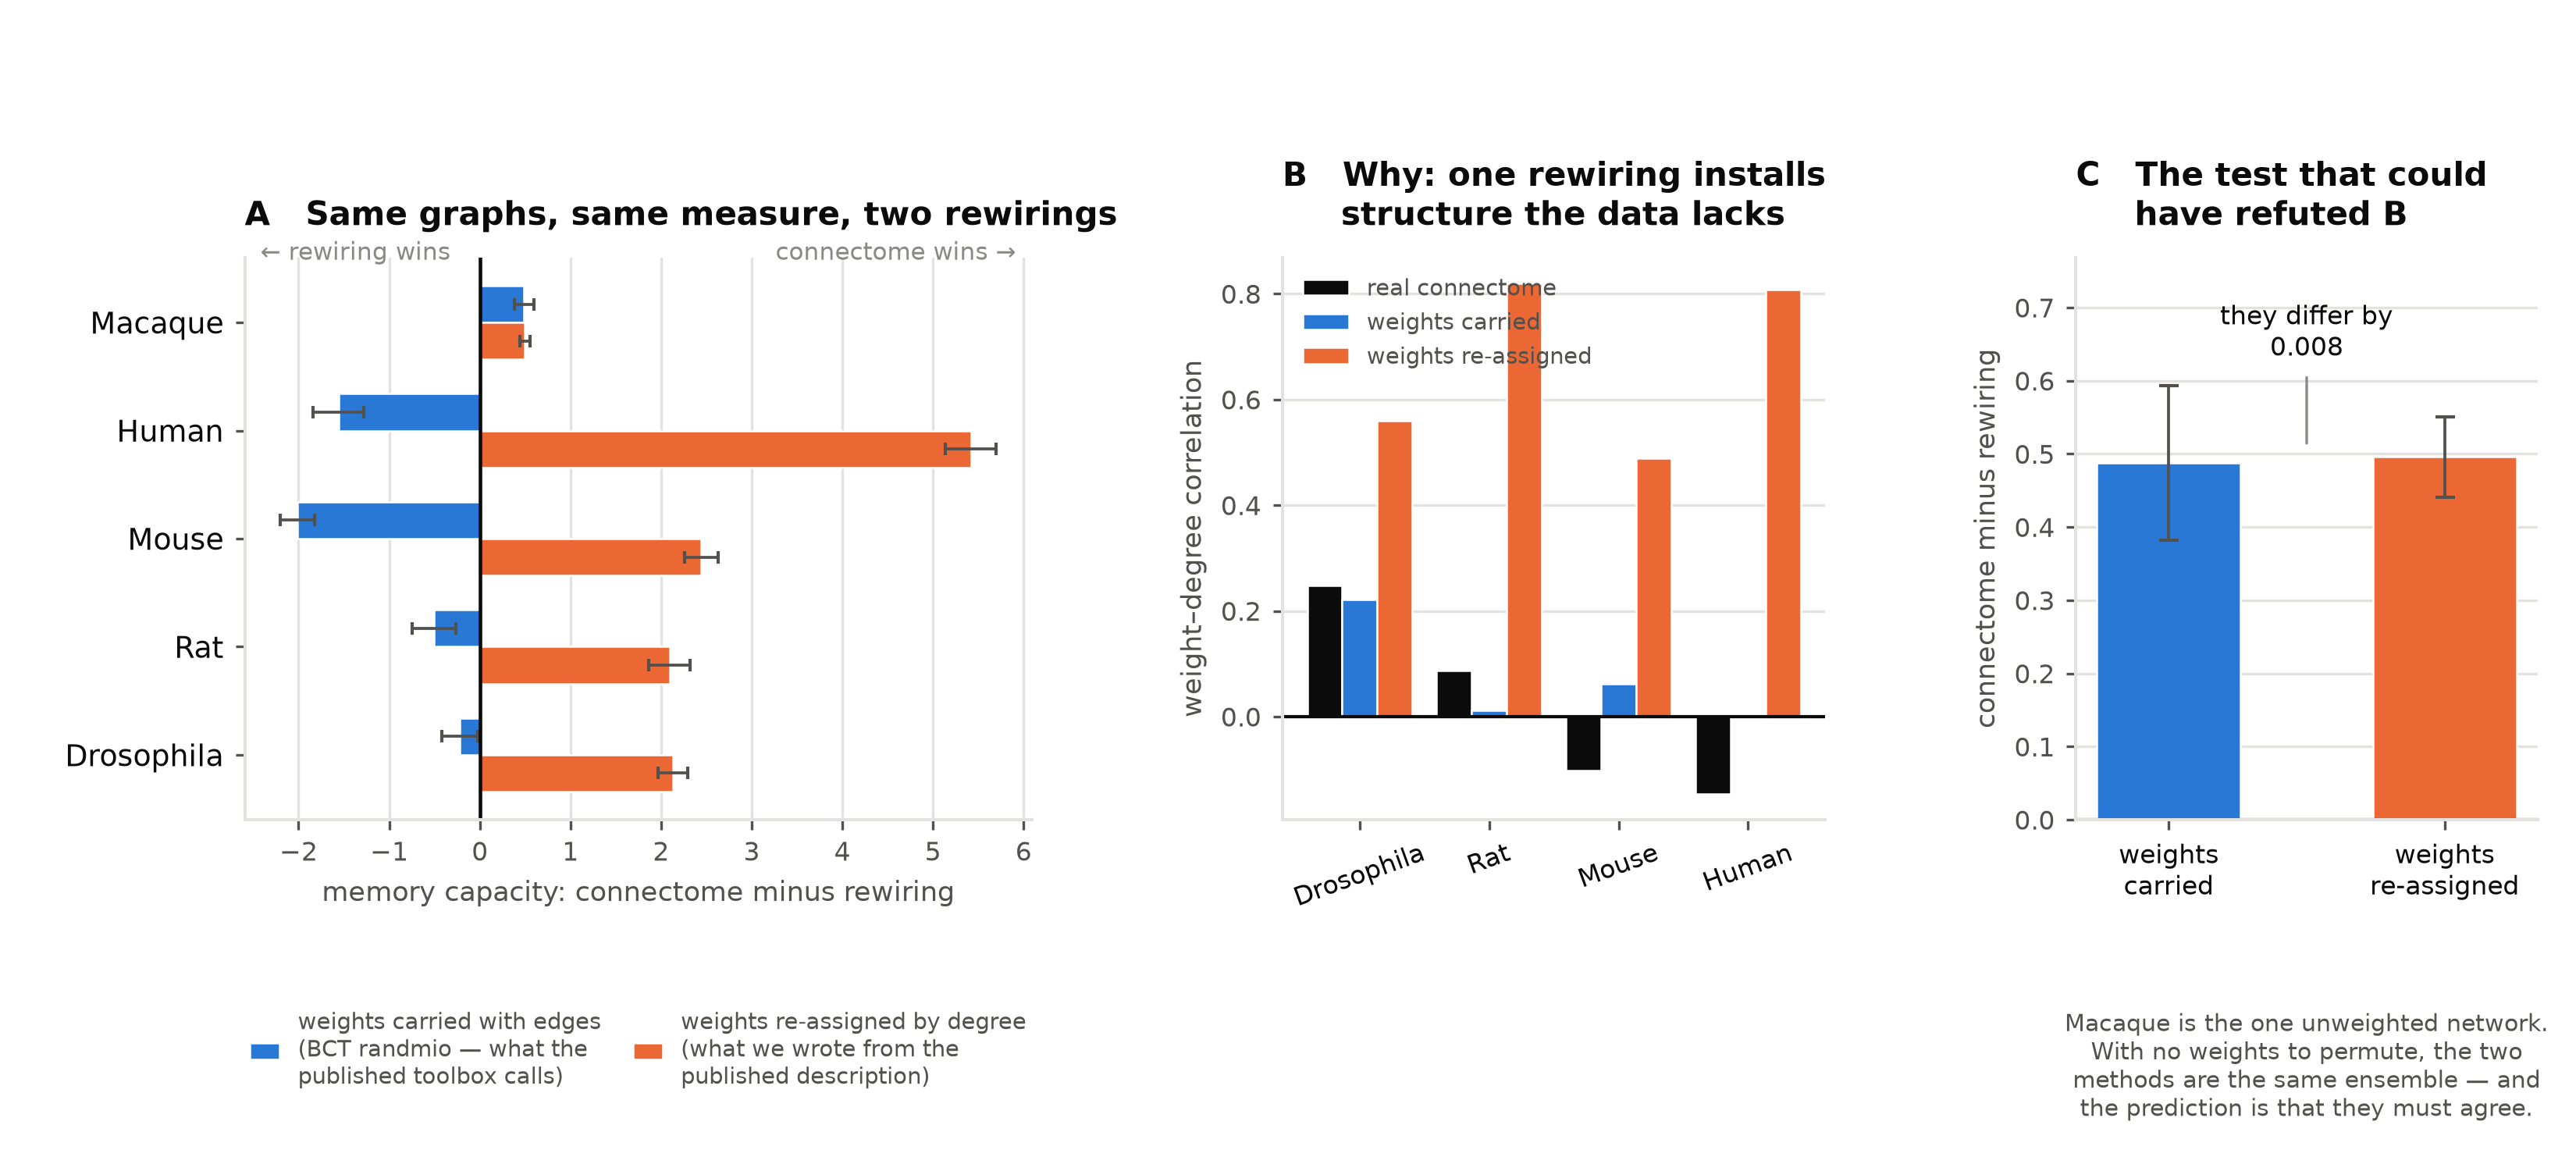
\includegraphics[width=0.98\textwidth]{figures/fig_null_choice.png}
\caption{\textbf{Two rewirings that answer to the same description, and the answers they
give.} \textbf{(A)} The empirical connectome's memory-capacity advantage over each of two
degree-preserving rewirings, at $\rho = 1$, with graded units. Same graphs, same inputs,
same delays, same readout, ten paired instances, 95\% confidence intervals. The only thing
that differs between a blue bar and the orange bar beside it is what happened to the edge
weights during randomisation: carried along with their edges, or re-assigned to the
rewired graph by endpoint-degree rank. Both procedures preserve the degree sequence and
the weight distribution exactly, and both are described in the literature as
``degree-preserving randomisation''. In four of five networks the pair points in opposite
directions. \textbf{(B)} The reason. Rank-reassignment does not only randomise: it
installs an association between an edge's weight and its endpoints' degrees that the
empirical graphs do not have (black) and that weight-carrying rewiring does not create
(blue). A reservoir whose largest weights sit on hub-to-hub edges is a poor one, so the
connectome's measured advantage over it is inflated. \textbf{(C)} The observation that
makes (B) an explanation rather than a story, because it could have come out the other
way. If the difference arises from permuting weights, then on a network with no weight
variation the two procedures are the same ensemble and must agree. Macaque is unweighted.
There the two measured advantages differ by $0.008$ capacity units, against a median
disagreement of $\NullDisagreeMedian$ across the rest of the set.}
\label{fig:nullchoice}
\end{figure*}

\begin{table*}[t]
\centering\small
\caption{\textbf{The connectome advantage depends on which rewiring it is compared
against, and on what a unit is.} Empirical connectome against two degree-preserving
rewiring ensembles at $\rho = 1$, the operating point of the published comparison, on the
five regional connectomes distributed with \texttt{conn2res}. \texttt{randmio} carries
each weight along with its edge; rank-reassignment rewires the topology and then
re-assigns the same multiset of weights by endpoint-degree rank. Both satisfy
``degree-preserving randomisation''. Identical graphs, inputs, delays and readout; ten
paired instances; paired $t$-test, $\ast$ marks $p < 0.05$. Absolute capacities are shown
because they establish whether a cell is informative: the human spiking row sits at the
floor and carries nothing, the other four do not.}
\label{tab:unitmodel}
\resizebox{\textwidth}{!}{%
\begin{tabular}{lrrrrr}
\toprule
& \textbf{Connectome} & \multicolumn{2}{c}{\textbf{BCT} \texttt{randmio}} & \multicolumn{2}{c}{\textbf{Rank-reassigned}} \\
\cmidrule(lr){3-6}
\textbf{Network} & \textbf{Capacity} & \textbf{Capacity} & \textbf{Difference} & \textbf{Capacity} & \textbf{Difference} \\
\midrule
\multicolumn{6}{l}{\emph{Graded-rate units} (\texttt{tanh})} \\
\quad Human & 11.46 & 13.02 & -1.56\,$\pm$\,0.28$^{\ast}$ & 6.04 & +5.42\,$\pm$\,0.28$^{\ast}$ \\
\quad Macaque & 8.67 & 8.19 & +0.49\,$\pm$\,0.11$^{\ast}$ & 8.18 & +0.50\,$\pm$\,0.06$^{\ast}$ \\
\quad Mouse & 7.19 & 9.20 & -2.01\,$\pm$\,0.19$^{\ast}$ & 4.75 & +2.44\,$\pm$\,0.19$^{\ast}$ \\
\quad Rat & 7.46 & 7.97 & -0.51\,$\pm$\,0.24$^{\ast}$ & 5.37 & +2.09\,$\pm$\,0.22$^{\ast}$ \\
\quad \textit{Drosophila} & 5.92 & 6.14 & -0.22\,$\pm$\,0.20 & 3.79 & +2.13\,$\pm$\,0.16$^{\ast}$ \\
\multicolumn{6}{l}{\emph{Spiking units} (LIF)} \\
\quad Human & 0.05 & 1.36 & -1.31\,$\pm$\,1.29 & 0.02 & +0.03\,$\pm$\,0.05 \\
\quad Macaque & 1.93 & 1.88 & +0.04\,$\pm$\,0.07 & 1.94 & -0.01\,$\pm$\,0.04 \\
\quad Mouse & 1.34 & 1.61 & -0.27\,$\pm$\,0.08$^{\ast}$ & 1.56 & -0.23\,$\pm$\,0.11$^{\ast}$ \\
\quad Rat & 1.22 & 1.20 & +0.02\,$\pm$\,0.05 & 1.16 & +0.06\,$\pm$\,0.07 \\
\quad \textit{Drosophila} & 1.09 & 1.09 & +0.00\,$\pm$\,0.01 & 0.97 & +0.12\,$\pm$\,0.25 \\
\bottomrule
\end{tabular}}
\end{table*}


Every comparison in this literature is a comparison against a rewiring, and the rewiring
is almost always specified in a phrase: \emph{degree-preserving randomisation}, or
\emph{randomised while preserving density and degree sequence}. That phrase does not
determine an ensemble. At least two constructions satisfy it, and they differ in what
happens to the weights:

\begin{itemize}[leftmargin=1.2em,itemsep=2pt,topsep=3pt]
\item \textbf{Weight-carrying rewiring.} Double-edge swaps move edges, and each weight
travels with the edge that carries it. The Brain Connectivity Toolbox routine
\texttt{randmio\_und\_connected} / \texttt{randmio\_dir\_connected}
\cite{rubinov2010complex,maslov2002specificity} does this, additionally rejecting swaps
that disconnect the graph. This is what \texttt{conn2res} calls, and therefore what the
published result was measured against.
\item \textbf{Rank-reassigned rewiring.} The binary topology is randomised by the same
swaps, and the original multiset of weight values is then re-assigned to the new edges in
order of endpoint-degree product. This preserves the degree sequence and the weight
\emph{distribution} exactly, and destroys the association between a weight and the edge
carrying it.
\end{itemize}

Both are defensible nulls and both answer to the published phrase. We wrote the second
one, believing we had written the first, and the error is instructive enough that we ran
both rather than deleting it: it preserves every marginal the description names, it
produced a clean and highly significant result, and nothing about its output indicated
that it was answering a different question. It was caught by reading the toolbox source,
not by anything in the numbers.

\paragraph{The two ensembles do not agree.}
Figure~\ref{fig:nullchoice}A shows the result and Table~\ref{tab:unitmodel} the full
design against both. Of $\NNullCells$ (network,
unit model) cells, the two nulls give the connectome's advantage \emph{opposite signs} in
$\NNullSignFlip$, and opposite \emph{significant} verdicts --- one says the connectome
leads, the other says it trails, both at $p < 0.05$ --- in $\NNullVerdictFlip$. The median
absolute disagreement between the advantage measured against one null and against the
other is $\NullDisagreeMedian$ capacity units, and the largest is $\NullDisagreeMax$. For
scale, these are differences of the same order as the effects the literature reports.

\paragraph{Which one reproduces the published direction.}
Against the weight-carrying ensemble --- the one the original toolbox builds --- the
graded-rate reservoir puts the connectome ahead in $\NBctRateLeads$ of
$\NBctRateNetworks$ networks and behind in $\NBctRateTrails$, median
$\BctRateMedian$. Against the rank-reassigned ensemble the same graphs, the same unit
model and the same operating point put it ahead in $\NRankRateLeads$ of
$\NRankRateNetworks$, median $\RankRateMedian$. The direction of the headline result in
this design is set by a choice that the method sentence does not record.

\paragraph{Why they differ, and a prediction that could have refuted it.}
The disagreement is not noise, and it has a structural cause specific enough to be
checked in advance (Fig.~\ref{fig:nullchoice}B,C). Sorting the weight multiset onto rewired edges by endpoint-degree
product does not merely randomise: it \emph{installs} an association between an edge's
weight and its endpoints' degrees. Across the $\NNullWeighted$ weighted networks,
carrying weights with their edges shifts the weight--degree correlation by a median of
$\NullShiftBct$ relative to the empirical graph, and never by more than
$\NullShiftBctMax$; rank-reassignment shifts it by $\NullShiftRank$. In mouse the
empirical association is slightly \emph{negative} ($\WDegMouseEmp$), \texttt{randmio}
returns $\WDegMouseBct$, and rank-reassignment returns $\WDegMouseRank$; in rat the
corresponding figures are $\WDegRatEmp$, $\WDegRatBct$ and $\WDegRatRank$. A null that
adds a property the data lacks is not a control for the absence of that property, and a
reservoir whose largest weights are concentrated on hub-to-hub edges is a poor one --- so
the connectome's advantage over it is inflated, in the direction and roughly the
magnitude we observed.

This account makes a prediction that would have falsified it cheaply: if the difference
comes from permuting weights, then on a network with no weight variation the two
constructions are the same ensemble and must agree exactly. One network in the set is
binary. On macaque the two nulls shift the weight--degree association by
$\WDegMacaqueBct$ and $\WDegMacaqueRank$ respectively --- that is, by nothing --- and
the connectome's measured advantage against them differs by $0.008$ capacity units,
against a median disagreement of $\NullDisagreeMedian$ elsewhere. It is the one cell in
Table~\ref{tab:unitmodel} where the choice of null provably cannot matter, and it is the
one cell where it does not.

\paragraph{What this does and does not establish.}
It does not show that either null is wrong. Rank-reassignment is a coherent ensemble and
a comparison against it is a coherent question --- it asks whether the \emph{placement} of
a connectome's weights matters given its degree sequence, which is a narrower and in some
ways sharper question than the one weight-carrying rewiring asks. What it shows is that
the two questions have different answers, that the phrase in general use does not
distinguish them, and that a reader cannot recover which was asked from the reported
number. A replication that constructs its own null from the published description is
therefore not a replication, and we include ours as an instance of that failure rather
than a warning about it.

\subsection{What a firing threshold does to the comparison}
\label{sec:res-unit}

The disagreement of \S\ref{sec:res-operating} has a candidate explanation that does not
involve the operating point at all, and it is checkable in one experiment.
\cite{suarez2024connectome} evaluate an echo state network of $\tanh$ units. We evaluate
a spiking leaky integrate-and-fire network. Those are not two implementations of one
model. A $\tanh$ unit responds to any input however small and is never silent; a LIF unit
below threshold emits nothing and contributes no variance to the readout at all.

We therefore ran both unit models over identical graphs, identical rewirings, identical
inputs, identical delays and an identical readout, on the five regional connectomes
distributed with \texttt{conn2res} --- the networks the published claim is made on, so
that the comparison inherits neither our subgraph extraction nor our binarisation.
$\NUnitEvaluations$ evaluations: $\NUnitNetworks$ networks $\times$ $\NUnitInstances$
paired instances $\times$ $\NUnitGains$ gains $\times$ two unit models.

All numbers in this subsection are measured against \texttt{randmio}, the ensemble the
published toolbox builds, for the reasons given in \S\ref{sec:res-nullchoice}.

\paragraph{With graded units, against the published null, we do not recover the published
direction.}
The empirical connectome leads its rewiring in $\NBctRateLeads$ of $\NBctRateNetworks$
networks at $\rho = 1$ and \emph{trails} significantly in $\NBctRateTrails$, median
$\BctRateMedian$ capacity units. Against the rank-reassigned ensemble, on the same graphs
at the same operating point in the same unit model, it leads in $\NRankRateLeads$ of
$\NRankRateNetworks$, median $\RankRateMedian$.

We do not read this as a refutation of \cite{suarez2024connectome}. Our harness differs
from theirs in the input projection, the delay set and the ridge solver as well as the
null, and any of those could account for a reproduction failure. What it does establish
is narrower and, we think, more useful: the choice of null \emph{alone} moves the result
by more than the effect being reported, which makes it a sufficient explanation for a
disagreement of this size without anything else having to be wrong. A reproduction
attempt that differs from the original in its null is not evidence against the original.

\paragraph{With spiking units the comparison is weaker still.}
On the same graphs the connectome leads significantly in $\NUnitSpkLeads$ of
$\NUnitSpkNetworks$ networks at $\rho = 1$ and trails significantly in
$\NUnitSpkTrails$; the median difference is $\UnitSpkMedianDiff$. Across the gain axis it
leads in $\UnitSpkFracLeadsAllGains$ of cells. Capacity itself falls by a factor of
$\UnitCapRatio$, from $\UnitCapRate$ to $\UnitCapSpiking$, so part of the weakening is
simply that there is less signal to resolve --- and the next paragraph asks whether the
rest is a fact about spiking units or about our choice of constants.

\paragraph{Is the spiking model simply untuned?}
The obvious objection is that we ran the spiking reservoir at one threshold, one leak and
one input scale, none of them tuned, and that a quiet network is a misconfigured one
rather than an informative one. That objection deserves an experiment rather than a
paragraph, and it gets one designed to refute us: we swept input gain from $\TuneGainLo$
to $\TuneGainHi$, threshold from $\TuneThreshLo$ to $\TuneThreshHi$ and two leaks ---
$\NTuneConfigs$ configurations, $\NTuneEvaluations$ evaluations --- and asked whether the
connectome advantage appears \emph{anywhere} the network is computing.

It does, in a few places, and not enough of them to sustain the strong claim. Of
$\NTuneCells$ (network, configuration) cells, $\NTuneHealthy$ are healthy by the
pre-stated criterion that the rewired control retains capacity above $0.5$ with fewer
than 80\% of units silent. Among those, the connectome leads significantly in
$\NTuneLeads$ and \emph{trails} significantly in $\NTuneTrails$, with a median difference
of $\TuneMedianDiff$. The configuration used in Table~\ref{tab:unitmodel} is not a
pathological corner: it sits within 20\% of the best capacity the sweep found.

So the accurate statement is not that the advantage is absent under spiking units but
that it is \emph{sporadic and inconsistent in sign} --- present in $\NTuneLeads$ of
$\NTuneHealthy$ well-conditioned settings, reversed in more of them, and negative at the
median. That is a weaker claim than the one we set out to make, and it is weaker in the
same direction as everything else in this section: once the null is the published one,
the unit model is no longer carrying a clean reversal, because there is no longer a clean
effect in either model for it to reverse.

\paragraph{The silencing mechanism, which we had previously reported as refuted.}
We predicted the mechanism before running it: a heavy-tailed degree sequence should leave
a connectome's low-degree neurons below threshold, silencing them, while no $\tanh$ unit
can be silent. The silencing is real and large --- $\UnitDeadSpiking$ of spiking units
never fire, against $\UnitDeadRate$ of rate units. Whether it is also \emph{differential}
is a question the choice of null decides, and we have had both answers. Against the
rank-reassigned ensemble the silencing gap did not predict the capacity gap and we
reported the prediction as failed. Against \texttt{randmio} it does: across
$\UnitSilenceGapN$ (network, gain) cells, the amount by which a connectome silences more
than its rewiring predicts the amount by which it loses capacity,
$r = \UnitSilenceGapR$, $p = \UnitSilenceGapP$.

We report the sign change rather than only the surviving result, because the two
conclusions were drawn from the same code and the same graphs and differ only in the
control. The supported version is the one measured against the published ensemble, and it
is a modest claim: differential silencing accounts for part of the spiking arm's
behaviour, in the predicted direction, leaving most of the variance unexplained.
Thresholding also compresses the measurement for every topology alike --- mean capacity
falls from $\UnitCapRate$ to $\UnitCapSpiking$, a factor of $\UnitCapRatio$ --- and that
compression is not differential at all.

\paragraph{A floor, declared.}
For the human network the spiking capacities are $0.049$ against $0.019$ --- both
effectively zero, so that network is uninformative in the spiking arm whatever it shows.
The remaining four retain capacities between $1.0$ and $1.9$ and do carry information.
The claim rests on those four.

\paragraph{What this licenses.}
Less than we hoped, and something worth saying anyway. We cannot claim a clean reversal
between unit models, because against the published null there is no clean effect in the
graded model to reverse. What we can claim is that the two model classes do not give the
same answer on identical graphs, that capacity in the spiking model is compressed by a
factor of $\UnitCapRatio$ so that effects of the reported size are near the resolution of
the measurement there, and that part of the difference tracks differential silencing. The
practical consequence is unchanged by the weakening: the connectome-reservoir result is
routinely invoked as motivation for neuromorphic architectures, neuromorphic hardware is
spiking, and the evidence that the property survives the transfer does not exist in
either direction yet.

\subsection{The contrast changes sign along the gain axis}
\label{sec:res-operating}

\begin{figure*}[t]
\centering
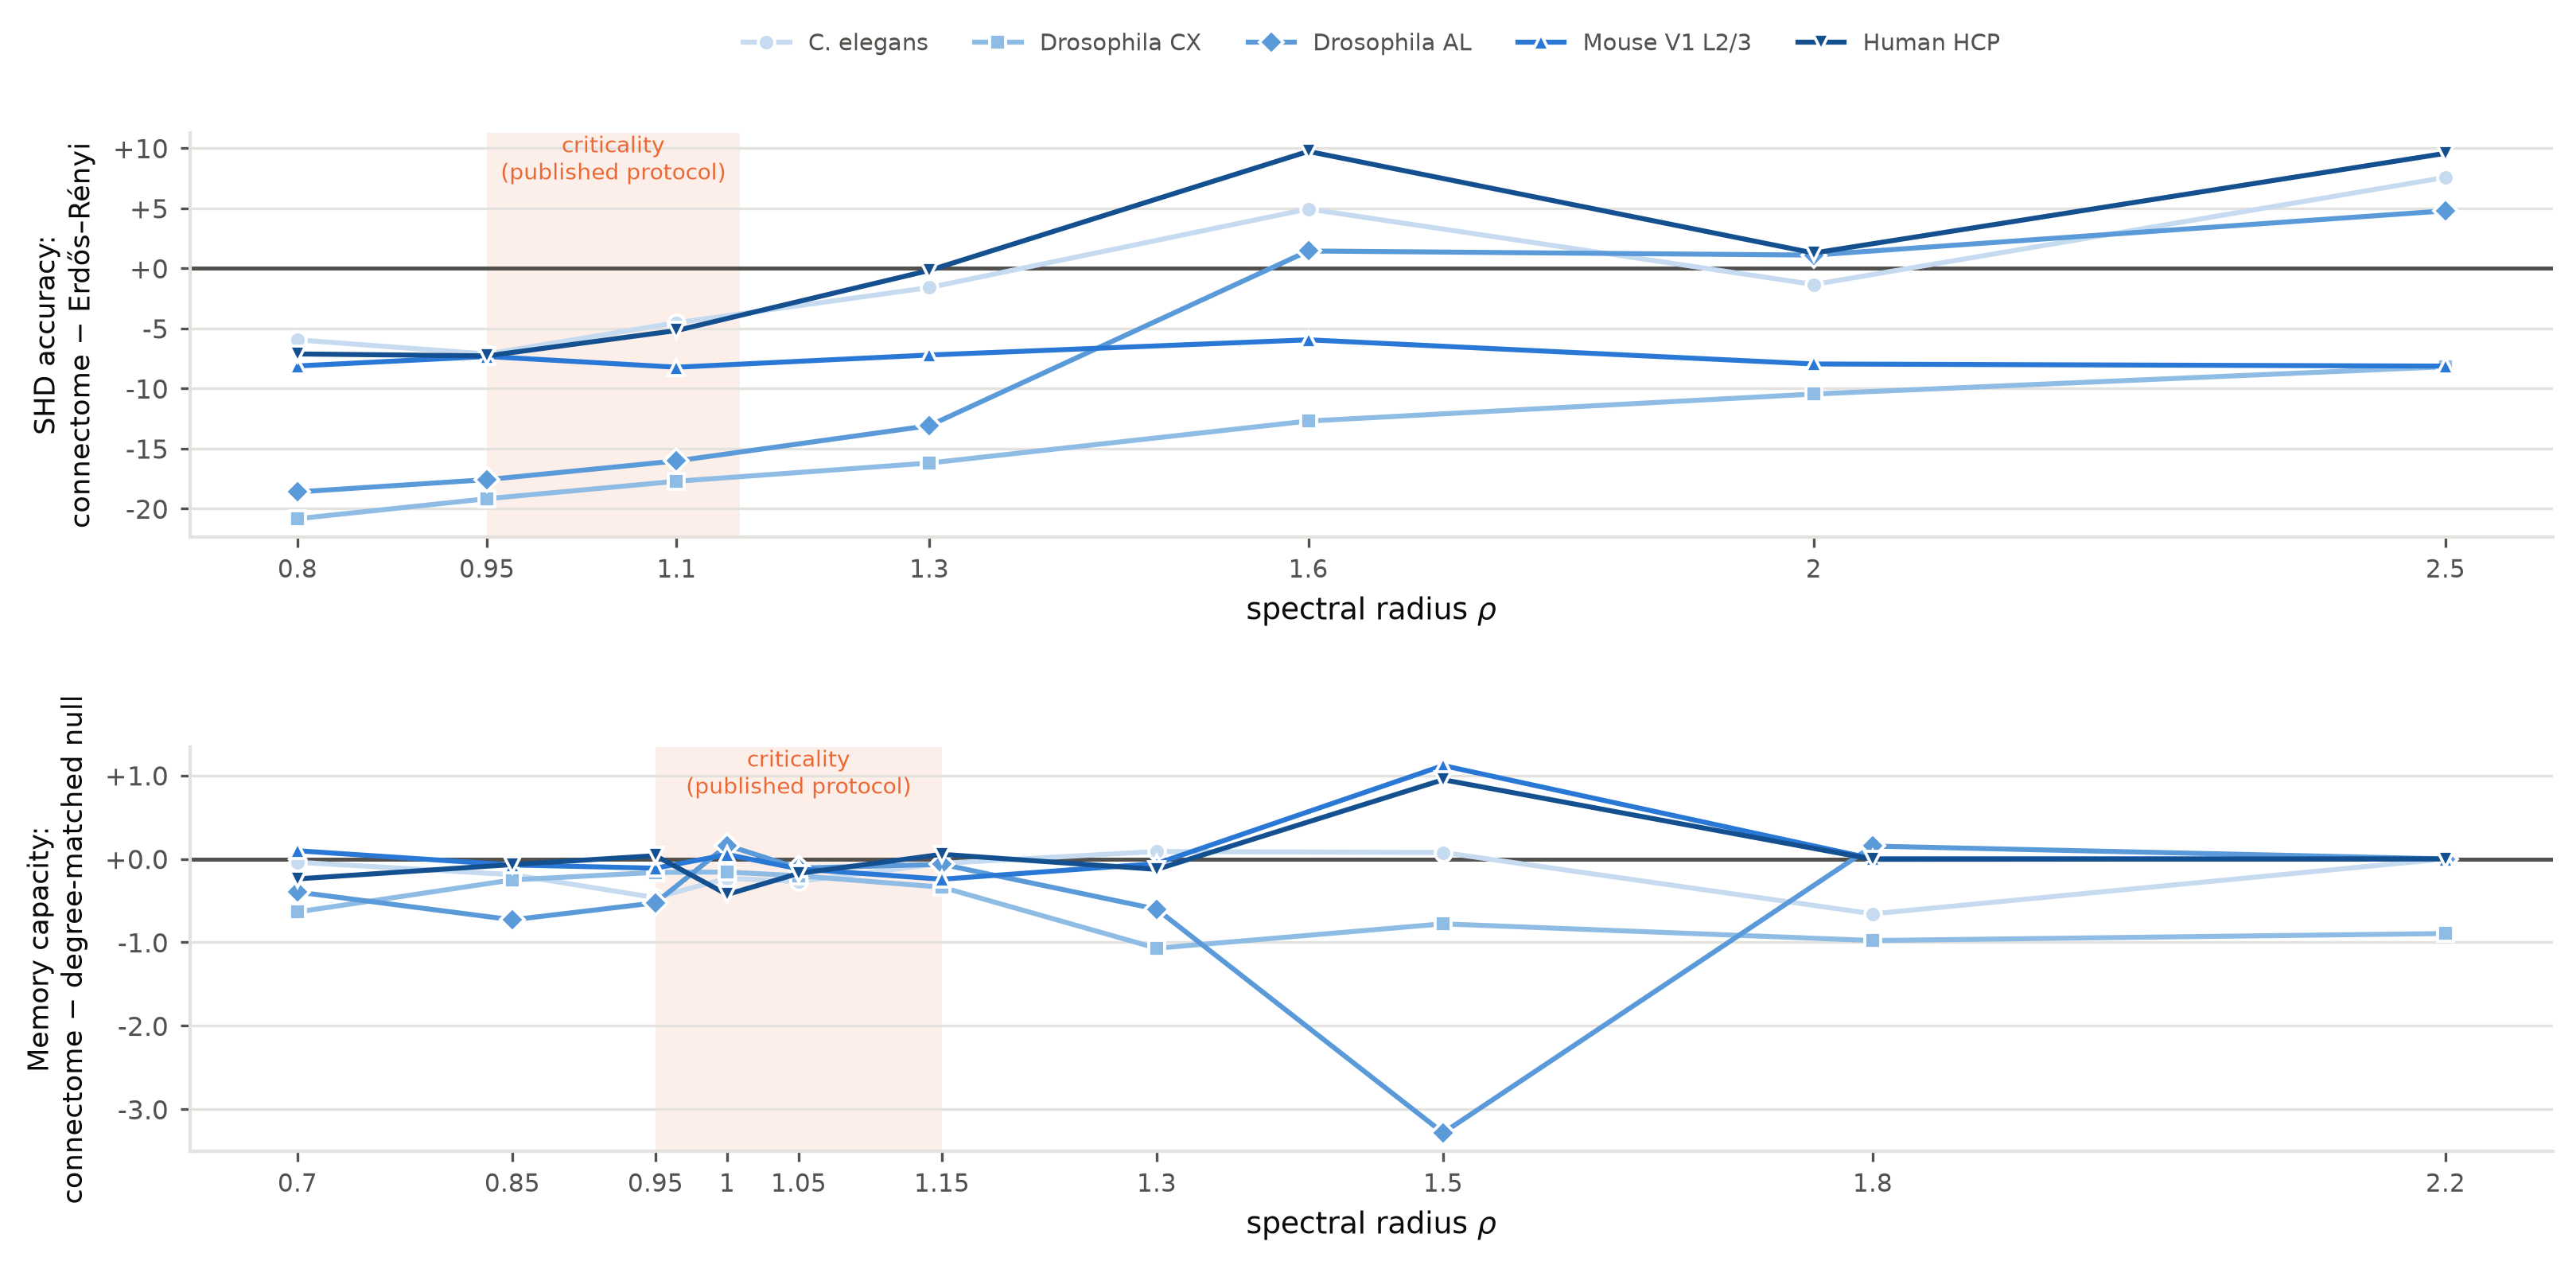
\includegraphics[width=0.95\textwidth]{figures/fig_operating_point.png}
\caption{\textbf{Where the comparison is made decides what it finds.} Both panels plot a
\emph{contrast}, not a performance curve, so that zero is the line that matters: below it
the connectome leads, above it the null does. \textbf{Top:} SHD accuracy, empirical
connectome minus the Erd\H{o}s--R\'enyi rung. \textbf{Bottom:} linear memory capacity,
empirical connectome minus the degree-preserving null --- the quantity and the control
used by \cite{suarez2024connectome}. The shaded band marks the critical region
($\rho \approx 1$) at which that comparison is reported. A published result of this kind
is a single point on one of these curves.}
\label{fig:operating}
\end{figure*}

Everything reported so far was measured at one operating point. \S\ref{sec:res-rate}
showed that the choice of operating point is not innocuous even when spectral radius is
held fixed. The question this raises is sharper than a robustness check, because the
literature reaches the opposite conclusion to ours on closely related measurements, and
does so at a different point on the same axis.

Su\'arez et al.~\cite{suarez2024connectome} report that empirical connectomes have significantly greater
linear memory capacity than degree-preserving rewirings, and report it \emph{at
criticality}, at a spectral radius of $1$. Our ladder is evaluated at
$\rho = \SpectralRadius$ and finds the opposite, on that same probe
(\S\ref{sec:res-dynamics}). Both measurements can be right, and we show that they are: the
contrast is not a fixed property of the pair of graphs being compared. It changes sign
along the gain axis.

\paragraph{Sweeping the axis.}
We re-ran the full ladder across $\NGainPoints$ spectral radii from $\GainGridLo$ to
$\GainGridHi$, $\NinstancesGain$ surrogates per rung per gain, each surrogate swept across
the whole axis so that curvature in $\rho$ is not confounded with surrogate-to-surrogate
variation. Of $\NGainCells$ evaluations $\NGainCellsFailed$ failed and are excluded and
counted rather than averaged in.

Two things follow, and the first is not what we expected to find.

\emph{On task accuracy the published direction does not appear, at any operating point we
tested including criticality.} At $\rho = \RhoCritical$ the Erd\H{o}s--R\'enyi rung leads
the empirical connectome in $\NGainNullLeadsAtCritical$ of $\NGainNetworks$ networks, with
every one of those differences significant against its own paired instance variation;
the median gap is $\GapAtCritical$. At $\rho = \RhoOurs$ it is $\GapAtOurs$. Whatever
advantage connectome topology has at criticality, it is not visible in the accuracy of a
linear readout on this task.

This is consistent with what has recently been reported from a hyperparameter sweep of
the \textit{C.\ elegans} connectome against Erd\H{o}s--R\'enyi, Watts--Strogatz and
shuffled controls \cite{hyperparam2026determinants}, which finds the connectome in a
lower-peak-performance, lower-sensitivity regime and notes that the
connectome-versus-null contrast varies with raw spectral radius. Our contribution on this
point is not the variation, which that work identifies, but its extent.

\emph{The contrast is not merely gain-dependent; it is not a constant of the pair being
compared.} It changes sign
along the axis in $\NGainSignFlip$ of $\NGainNetworks$ networks, with the contrast
significant on both sides of the crossing in each case, and the largest within-network
swing is $\GapSwingMax$ of accuracy --- several times the size of any structural effect in
\S\ref{sec:res-ladder}. In those networks the connectome catches the unstructured rung and
overtakes it above $\rho \approx 1.3$. In the remaining two the unstructured rung leads
significantly at every gain on the grid. We note the disagreement plainly:
\cite{hyperparam2026determinants} reports the connectome-versus-null relationship as
consistent across the regimes it tests, and we find a reversal. The two are not
straightforwardly comparable --- that work sweeps one connectome on task-agnostic probes,
ours sweeps five on task accuracy, and our own probe-based sweep is underpowered
(below) --- so we record this as a discrepancy to be resolved rather than as a
correction. The direction of the comparison is therefore a
joint property of the topology \emph{and} the regime, and a single number reported for it
is a number about both.

\paragraph{Attempting the published comparison directly, and failing to resolve it.}
The bottom panel of Figure~\ref{fig:operating} repeats the measurement the published claim
rests on: linear memory capacity, empirical connectome against a degree-preserving null,
across $\NMemGainPoints$ gains from $\MemGridLo$ to $\MemGridHi$, ten surrogates per rung
per gain, paired by instance.

We do not detect the reported advantage. At $\rho = \MemRhoCritical$ --- the published
operating point --- the connectome leads in $\NMemAdvPosAtCritical$ of $\NMemNetworks$
networks by the sign of the mean, and in $\NMemAdvSigAtCritical$ of $\NMemNetworks$ once
the paired confidence interval is taken into account. The median difference is
$\MemAdvAtCritical$ capacity units, against the null.

\emph{This is a non-detection and not a refutation, and the distinction is the whole of
it.} Our design at this operating point resolves a median effect of $\MemMDEMedian$
capacity units at $\PowerLevel$ power --- $\MemMDEFracMedian$ of the null network's own
capacity. An advantage of the size that would be scientifically interesting here is
comfortably inside our confidence intervals. On $\NMemPowered$ of $\NMemNetworks$
networks the variance is low enough to resolve $\MemMDEFracMin$ of capacity, and there
the difference is $+0.05 \pm 0.11$; on the other four the attempt is uninformative, and we
say so rather than reporting four null results as though they were evidence.

Several differences from the original could account for a real effect going undetected
here, and we have not isolated which. Our networks are size-matched induced subgraphs of
$\NnodesTarget$ nodes rather than whole released connectomes; our spiking reservoir is a
binary-weight LIF network rather than a rate model; and our memory-capacity estimator,
input scaling and washout are our own. We report the attempt because a reader deciding
what to believe about the published result should know that an independent implementation
did not see it, and should equally know that this implementation could not have seen it
unless it were very large.

\paragraph{Against an unstructured graph the direction is consistent.}
One asymmetry survives the power problem, because it is large. The published comparison
is against a \emph{degree-preserving} null. Against the Erd\H{o}s--R\'enyi rung the
connectome's memory capacity is lower at essentially every gain and in every network, by
margins that reach several capacity units --- far outside the intervals above. Whatever
the degree sequence and the wiring buy relative to each other, they do not recover what
is lost relative to an unstructured graph of the same size and density. This is the same
ordering the accuracy sweep gives, and the same one the ladder gives at a fixed gain.

\paragraph{Where the sweep stops being a comparison.}
A gain axis has an end, and past it the question dissolves. As $\rho$ grows the reservoir
saturates: every neuron fires at every step, the readout features stop varying, and the
state carries no information about the input regardless of how it is wired. We record the
effective rank of the readout features for every cell as a fraction of their number, so
that regime is identifiable by a number rather than inferred from a surprising accuracy.
It falls from $\FeatureRankAtOurs$ at $\rho = \RhoOurs$ to $\FeatureRankAtMaxGain$ at the
top of the grid. Of $\NGainCells$ evaluations, $\NGainCellsFailed$ failed outright and are
excluded and counted rather than averaged in as missing values.

We therefore do not rest the sign change on the saturated end of the axis. The crossing
reported above occurs between the critical region and $\rho = \RhoOurs$, where the state
is still high-rank in every network, and the far end of the sweep is shown for
completeness rather than used as evidence.

\paragraph{Two protocols, two questions.}
Neither way of choosing an operating point is wrong, and the difference between them is
not a matter of care. Comparing each network at its own optimum asks how good a topology
can be made to look when the rest of the model is tuned for it; comparing at a common
point asks what the topology does to a network held otherwise fixed. Under the first
protocol the rungs peak at different gains --- median $\BestRhoLzero$ for the
Erd\H{o}s--R\'enyi rung against $\BestRhoLfour$ for the connectome --- and the contrast at
each rung's own best gain is $\GapAtOwnOptimum$, negative in
$\NGapAtOwnOptimumNeg$ of $\NGainNetworks$ networks.

We draw a methodological conclusion rather than a biological one. A single-operating-point
comparison between a connectome and a null establishes a fact about that operating point.
Reported without the curve, it is indistinguishable from a fact about the topology, and
the two differ by a sign over a range of $\rho$ that any two groups might reasonably
choose differently. This applies to our own matched-gain and matched-rate results in
\S\ref{sec:res-ladder} and \S\ref{sec:res-rate} exactly as it applies to the literature's,
and it is the reason we report the axis rather than a point.

\subsection{The null result is not an artefact of the sampler}
\label{sec:res-robust}

Because L3 is produced by an annealed chain rather than by a construction with a proof
behind it, two objections have to be answered before a null L2--L3 contrast can be read
as a statement about motifs. Neither is addressed by the ensemble validation of
\S\ref{sec:res-null}, which establishes only that the chain hits its target,
randomises, and does not reproduce held-out structure.

The first is mixing. If the chain has not moved far enough, its surrogates retain memory
of where they started and a null contrast means only that the chain was too short. We
therefore re-ran the L3 rung over chain lengths from $\SweepGridLo$ to $\SweepGridHi$
sweeps, a factor of eight around the value used throughout. Mean accuracy moves by a
median of $\SweepMedianSpread$ across that range, and at most $\SweepMaxSpread$ on any
network ($\SweepMaxSpreadWhere$). The reference to judge that against is the
surrogate-to-surrogate standard deviation at a \emph{single} chain length, which has a
median of $\SweepWithinSD$: the variation attributable to an eightfold change in chain
length is of the same size as the variation between surrogates drawn at one setting. It
is also not a drift --- accuracy is non-monotonic in chain length in
$\NSweepNonMonotone$ of $\NSweepNetworks$ networks, which is the signature of a chain
that has stopped moving rather than one still travelling. Both are far below the degree-sequence effect the
ladder resolves. We read this as showing the result is not chain-length limited, not as
showing the chain has provably mixed.

The second is the starting point. The chain we use begins at the empirical connectome
and walks under the census constraint; the opposite construction begins at a fully
rewired graph and anneals towards the census. The two guarantee opposite things, and
where both reach the target they should agree. Of the $\NRandomStartTotal$ networks, the
random start converges on $\NRandomStartConverged$; restricted to those, the two
constructions differ in mean accuracy by at most $\InitMaxGap$. Where the random start
fails it fails by not reaching the census at all, which is the reason the empirical start
is used in the main text rather than a preference between two equally good options.

\subsection{The same decomposition on intrinsic dynamics}
\label{sec:res-dynamics}

A result read off a task metric invites the objection that the readout, not the
reservoir, is what is being measured. We therefore repeated the decomposition on three
task-independent probes of the reservoir itself --- linear memory capacity, kernel rank
and generalisation rank --- which are the standard measures of a reservoir's
computational capability and do not involve the benchmark at all. These were run at
$\NinstancesDyn$ surrogates per rung rather than $\NinstancesLadder$, so Holm correction
across the same $\NDynMemTotal$-contrast family is correspondingly harsher and the
significance counts are not comparable with those of \S\ref{sec:res-ladder}; the effect
sizes and the signs are.

\begin{figure}[t]
\centering
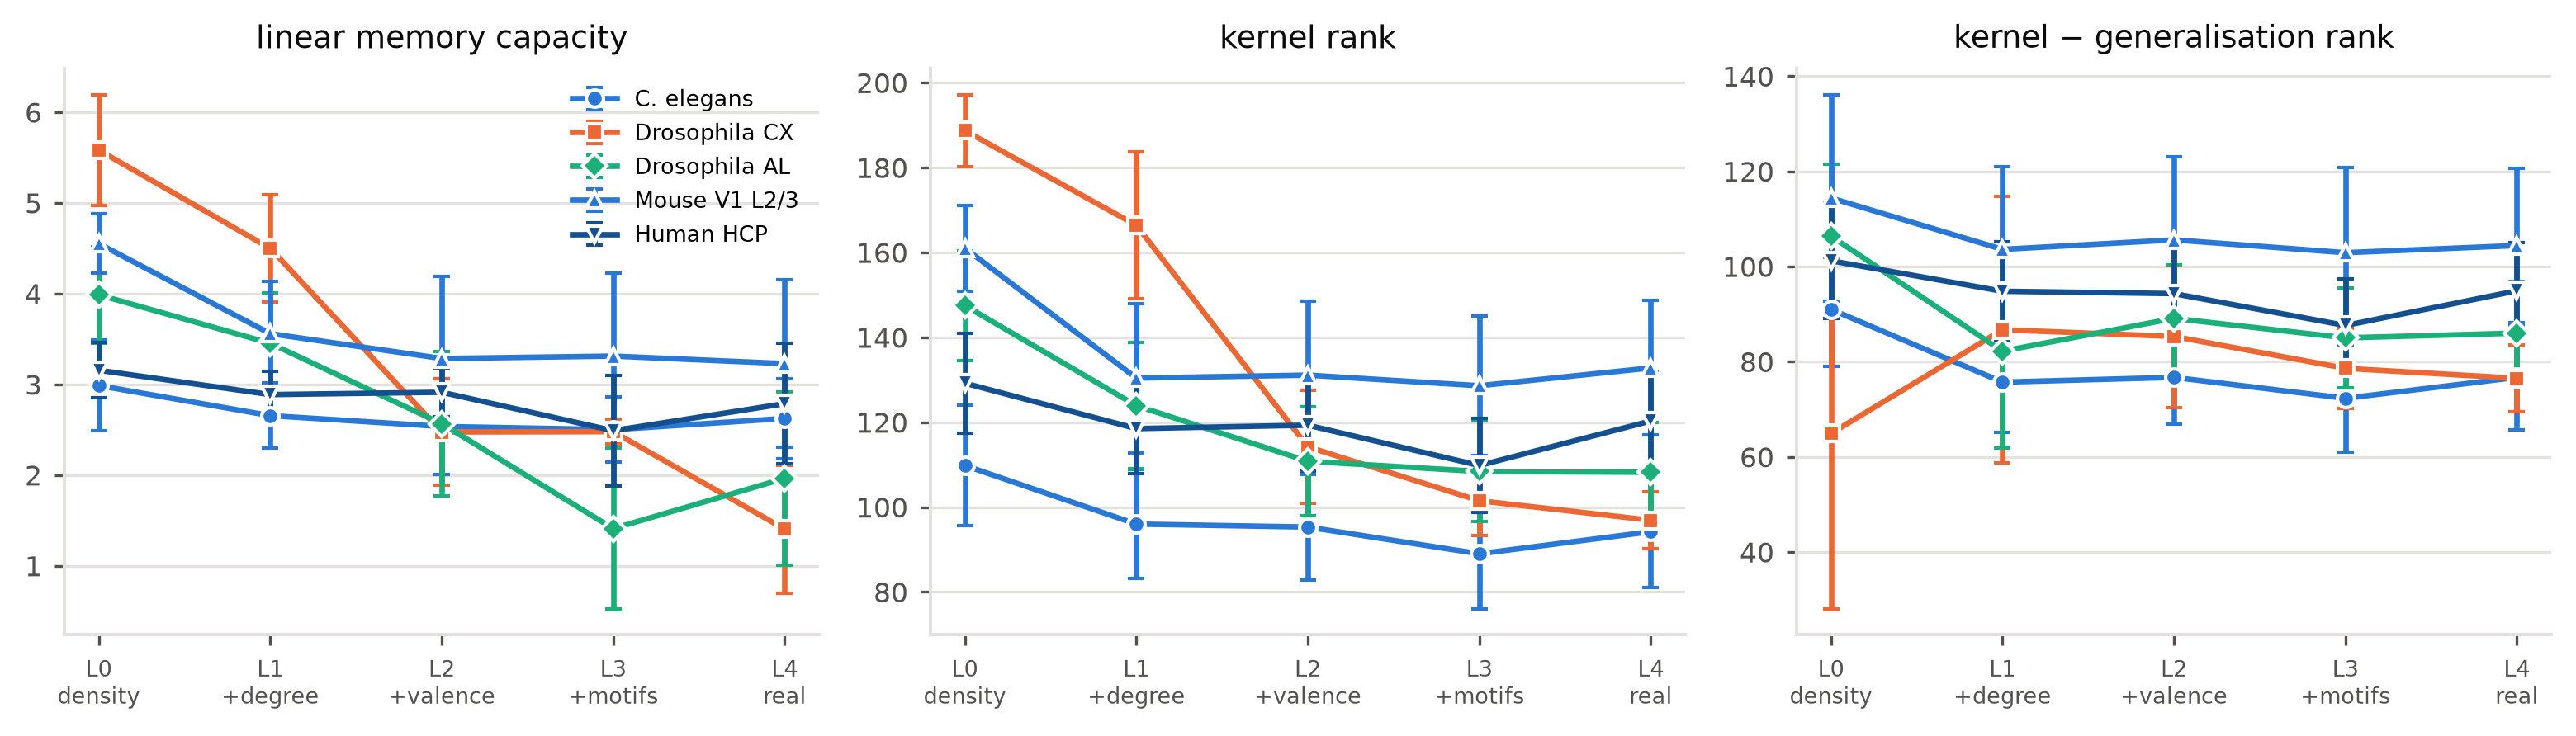
\includegraphics[width=\columnwidth]{figures/fig_dynamics.png}
\caption{\textbf{Dynamical probes across the ladder.} Memory capacity, kernel rank and
the capability index (kernel $-$ generalisation rank) as a function of ladder rung. The
probes are independent of the benchmark, and they reproduce its ordering: the
unstructured rung leads, and the decline is concentrated in the early rungs.}
\label{fig:dynamics}
\end{figure}

The probes reproduce the task result, including the part of it we did not expect
(Figure~\ref{fig:dynamics}). The Erd\H{o}s--R\'enyi rung has the higher memory capacity
in $\NDynMemLzeroHigher$ of $\NDynMemNetworks$ networks, by a median factor of
$\DynMemLzeroOverLfour$, and the higher kernel rank in $\NDynKernLzeroHigher$ of
$\NDynKernNetworks$, by $\DynKernLzeroOverLfour$. So the connectomes are not trading
task accuracy for some capability the benchmark fails to reward; they have less of the
capability the probes measure.

The ordering of properties also carries over. Imposing the degree sequence lowers memory
capacity in $\NDynMemDegreeNeg$ of $\NDynMemNetworks$ networks (median Hedges'
$g = \DynMemDegreeMedG$) and kernel rank in $\NDynKernDegreeNeg$ of
$\NDynKernNetworks$ ($g = \DynKernDegreeMedG$), while the motif census moves them least
of any rung ($g = \DynMemMotifMedG$ and $\DynKernMotifMedG$). After Holm correction
$\NDynMemSig$ of $\NDynMemTotal$ contrasts survive in memory capacity and
$\NDynKernSig$ of $\NDynKernTotal$ in kernel rank --- in both cases the same one, valence
placement in the \textit{Drosophila} central complex, the network whose edges are
two-thirds inhibitory.

The two classes of measurement agree on the direction --- every resolvable effect is
negative, and the unstructured rung leads --- and they agree that the degree sequence
carries the largest share. They do \emph{not} agree on the motif rung. On task accuracy
the motif census produces an effect comparable to the degree sequence's
($\MotifEffectMedian$ against $\DegreeEffectMedian$); on the dynamical probes it is the
smallest contrast in the ladder. We do not have an account of that divergence and do not
want to manufacture one. The most likely reading is that the probes measure properties of
the state ensemble that the ridge readout does not fully exploit, so a structural change
can cost task accuracy without costing measured capacity --- but that is a conjecture, and
the honest summary is that the benchmark and the probes concur on the headline ordering
and part company on one rung of it.

\subsection{Degeneracy is a property of directions}
\label{sec:res-degeneracy}

\begin{figure*}[t]
\centering
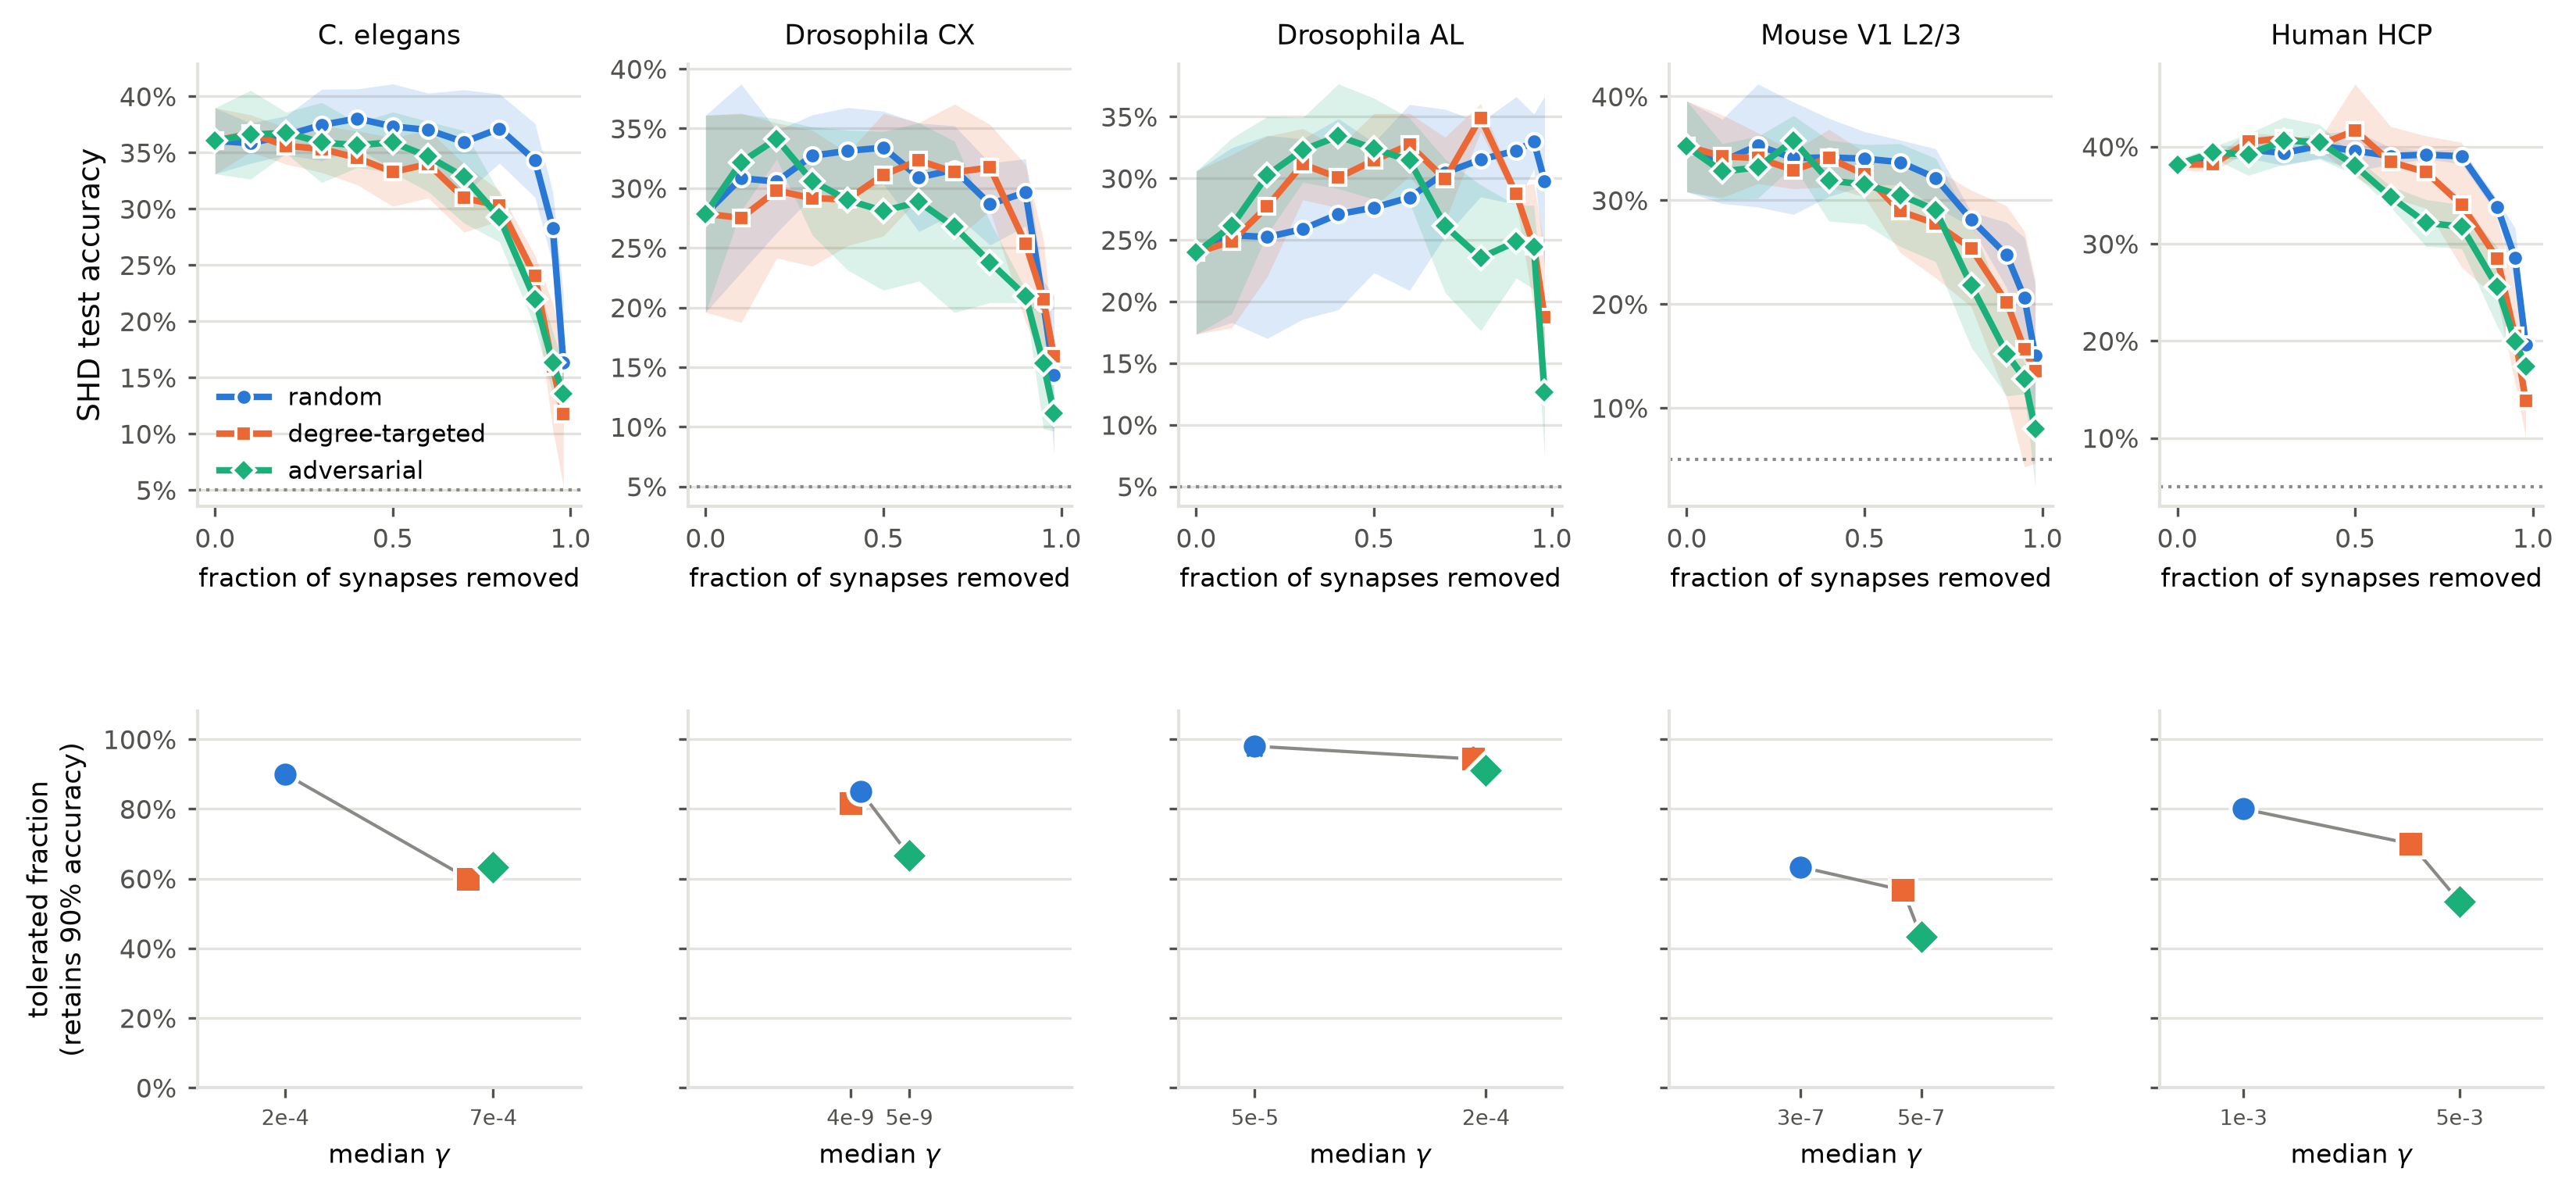
\includegraphics[width=0.95\textwidth]{figures/fig_pruning.png}
\caption{\textbf{Tolerance to synaptic removal depends on direction, not magnitude.}
\textbf{Top:} accuracy against the fraction of synapses removed, for uniformly random
pruning, degree-targeted pruning, and the first-order maximally damaging ranking, all at
matched spectral radius. \textbf{Bottom:} the ordinal prediction, tested within each network --- tolerated
fraction against median $\gamma$, one point per strategy. If tolerance falls with
$\gamma$ the three points descend left to right, which they do in
$\NGammaOrdered$ of $\NGammaNetworks$ networks. Note the $x$ ranges: $\gamma$ differs
between networks by five orders of magnitude, because it is normalised by a
network-specific worst-case constant, so these panels cannot be merged into one and
a pooled $\gamma$ axis would show nothing. Weight-magnitude
pruning is not shown because it is undefined on these graphs: the connectomes are
unweighted, so every edge has the same magnitude and a ``weakest-first'' schedule is an
index ordering in disguise.}
\label{fig:pruning}
\end{figure*}

The measured spectral gaps of these networks are as small as $\MinSpectralGap$, so the
Davis--Kahan bound admits perturbations of norm at most $\MaxDKAdmissible$ --- far below
any perturbation that a single synapse removal produces. The classical bound is not
loose here; it is inapplicable, and the ratio between empirical tolerance and that bound,
which an earlier revision of this work reported as evidence of biological robustness, is
a property of eigenvector conditioning.

Proposition~\ref{prop:tolerance} instead predicts that tolerance scales inversely with
the operational alignment $\gamma$ of the perturbation direction. We tested that in two
forms, and they do not give the same answer.

\paragraph{The ordinal prediction holds, mostly.}
Within each network, $\gamma$ is larger for the structured directions than for the
random one: relative to uniformly random removal, degree-targeted removal realises
$\GammaRelHub\times$ the worst case and the first-order maximally damaging ranking
$\GammaRelAdv\times$. The tolerated fractions run in the opposite order, as predicted ---
$\RNinetyRand$ for random removal, $\RNinetyHub$ for degree-targeted and $\RNinetyAdv$
for adversarial, a factor of $\RNinetyRatio$ between the extremes at identical
cardinality (Figure~\ref{fig:pruning}). Taken network by network, $\gamma$ orders the
three strategies correctly in $\NGammaOrdered$ of $\NGammaNetworks$.

\paragraph{The quantitative prediction does not.}
The proposition says more than an ordering: it says the tolerated magnitude scales as
$1/\gamma$, so the product $\gamma \cdot \|E\|_F^{\max}$ should be constant across
directions within a network. It is not. That product still varies by a median factor of
$\GammaProductSpread$ between strategies --- a reduction on the $\GammaRelAdv\times$
spread in $\gamma$ alone, but not the collapse the proposition predicts. We report this
as a partial failure of our own prediction rather than restricting the claim to the
ordering after the fact: $\gamma$ identifies which direction is more damaging, and does
not correctly predict by how much.

\paragraph{$\gamma$ is not comparable between networks.}
One property of $\gamma$ deserves emphasis because it is easy to misuse, including by
us. It is a realised fraction of a worst-case constant $C(T,a)$ that depends on
$\|A\|_2^{\,T}$, and across our five networks the median $\gamma$ spans a factor of
$\GammaSpanAcrossNetworks$. Absolute $\gamma$ values are therefore meaningful only
within a network, and pooled medians across networks --- which an earlier version of
this analysis reported --- are not a quantity at all. Every comparison above is made
within a network and then aggregated.

\paragraph{An unexpected feature of the survival curves.}
All three strategies \emph{improve} accuracy at low pruning fractions, peaking around
$40$--$60\%$ of synapses removed before declining (Figure~\ref{fig:pruning}). These
reservoirs are over-connected for the task, and the improvement is consistent with the
ladder's main finding: removing synapses attenuates exactly the degree heterogeneity
that the L0\,$\rightarrow$\,L1 contrast shows to be costly here. It also means the
tolerated fraction is a conservative summary, and that several random-pruning runs still
retain 90\% of unpruned accuracy at the largest fraction we tested, so $\RNinetyRand$ is
a lower bound.

This is the substantive point, and it survives the partial failure above. Robustness to
randomly chosen ablation is close to generic for large recurrent systems, because a
random direction is nearly orthogonal to any fixed functional subspace. Reporting it as
evidence of biological degeneracy overstates what has been shown: the same networks are
markedly more fragile to a perturbation of identical cardinality chosen along a damaging
direction. A degeneracy claim is only as strong as the worst direction it has been
tested against, and that conclusion needs only the ordering, which holds.

\subsection{What the accompanying hardware actually costs}
\label{sec:res-hardware}

\begin{table}[t]
\centering\small
\caption{\textbf{Logic synthesis of the accompanying RTL} with Yosys and ABC onto the
Nangate45 Open Cell Library (typical corner). These are the quantities this flow can
establish. No die area, power or energy-per-operation figure is reported: the flow
performs no placement, routing, clock-tree synthesis or parasitic extraction. No clock
frequency is reported either, because the toolchain ships no static timing analyser. The
commercial-process figures reported in earlier revisions of this project were never
measured and are withdrawn.}
\label{tab:synthesis}
\resizebox{\columnwidth}{!}{%
\begin{tabular}{lrrr}
\toprule
\textbf{Module} & \textbf{Cells} & \textbf{Flip-flops} &
\textbf{Cell area ($\mu$m$^2$)} \\
\midrule
\texttt{dendritic\_lif\_core} & 4,401 & 70 & 5,301 \\
\texttt{synaptic\_accumulator} & 19,649 & 8,192 & 63,361 \\
\texttt{aer\_crossbar\_router} & 39 & 17 & 124 \\
\texttt{cen\_accelerator\_top} & 590,116 & 25,644 & 749,263 \\
\bottomrule
\end{tabular}}
\end{table}


Table~\ref{tab:synthesis} reports logic synthesis of the accompanying RTL onto an open
cell library. We report gate count, flip-flop count and mapped pre-layout cell area, and
nothing else: this flow performs no placement, routing or parasitic extraction, so die
area and switching power are not determined by it, and it ships no static timing
analyser, so no clock frequency is claimed either. The commercial-process figures quoted in earlier revisions of this project --- a
28\,nm node, a die area, a picojoule-per-operation efficiency --- were produced by a
Python model with those values written in as constants, not by any synthesis flow, and
are withdrawn.
